\documentclass[12pt, letterpaper]{scrartcl}
\usepackage[utf8]{inputenc}
\usepackage{graphicx}
\usepackage{fancyhdr}
\usepackage{hyperref}
\usepackage{subfig}
\usepackage{float}

\usepackage{scalerel,amssymb}

\newcommand\equalhat{%
	\let\savearraystretch\arraystretch
	\renewcommand\arraystretch{0.3}
	\begin{array}{c}
		\stretchto{
			\scalerel*[\widthof{=}]{\wedge}
			{\rule{1ex}{3ex}}%
		}{0.5ex}\\ 
		=%
	\end{array}
	\let\arraystretch\savearraystretch
}

\pagestyle{fancy}
%\fancyhf{}
%\rhead{Share\LaTeX}
%\lhead{Guides and tutorials}
\lfoot{TUM - Computer Games Laboratory}
\rfoot{Page \thepage}
\cfoot{}

\hypersetup{
	colorlinks,
	citecolor=black,
	filecolor=black,
	linkcolor=black,
	urlcolor=black
}

\title{Solve'n Slide}
\subtitle{Project Notebook}
\author{Hanieh Arjomand-Fard\\Kevin Sawischa\\Markus Ansorge\\Stefan Aicher}
\date{30. April 2017}

\begin{document}
	
	\begin{titlepage}
		\maketitle
	\end{titlepage}
	
	\tableofcontents
	\newpage
	
	\section{Proposal}
	\subsection{Game Description}
	The goal of the game is to maneuver your character from your starting point to a finish line. The gameplay is divided into two main phases: the Manipulation-Phase and the Action-Phase. During the first phase the player has to manipulate the environment through different means in order to enable a successful playthrough of the level in the second phase. Throughout the Action-Phase the player must use the environment in combination with his sliding equipment to reach the goal. In order to achieve that he has to increase his speed to clear obstacles and avoid certain death.
	
	\subsubsection{Manipulation-Phase}
	This phase is the theoretical phase. The player will look in a top-down perspective on the terrain or fly as a camera through the level. The start and destination points are fixed. The destination point is not reachable in the first place. 
	The player needs to find the "optimal" path to reach the goal by altering the terrain itself. So the terrain is deformable at certain areas. Hills and valleys can be created by using a skill/gun that can raise or lower terrain parts. There is also the possibility of placing walls to run on or placing jump-pads and speed-boosters for refining speed more precisely. The player also needs to make sure to have enough fuel for his jetpack so there will be fuel tanks provided that can be picked up in the air. A further feature is to place explosives that can be triggered by the player during the action phase.
	\begin{figure}[ht]
		\centering
		\begin{tabular}{ccccc}
			\subfloat[Scale]{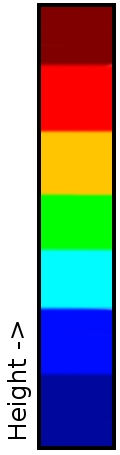
\includegraphics[scale=0.3]{images/HeightScale}}&&
			\subfloat[Increase and Decrease]{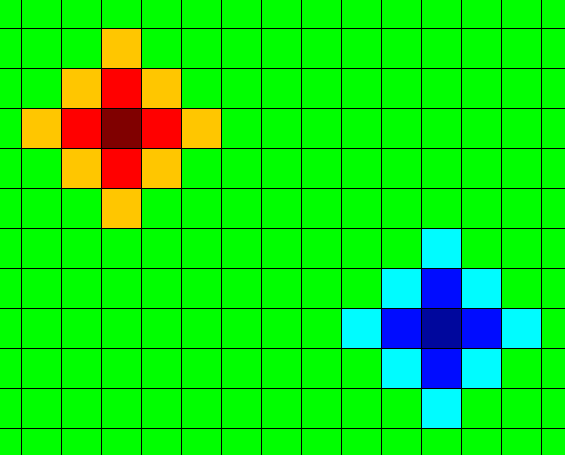
\includegraphics[scale=0.2]{images/Part1IncreaseAndDecreaseCharges}}&
			\subfloat[Decrease and Increase Combination]{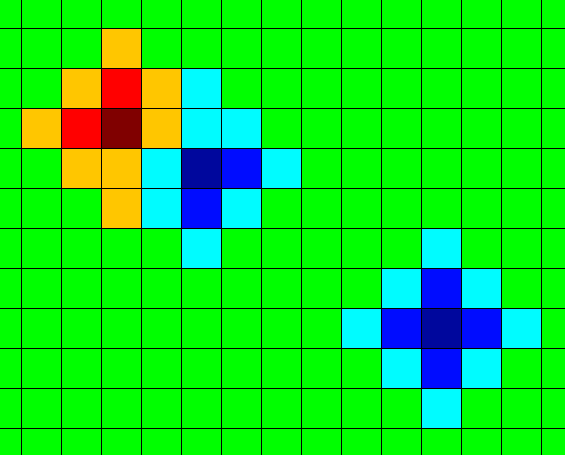
\includegraphics[scale=0.2]{images/Part2DecreaseCharge}}&
			\subfloat[Undo first Increase]{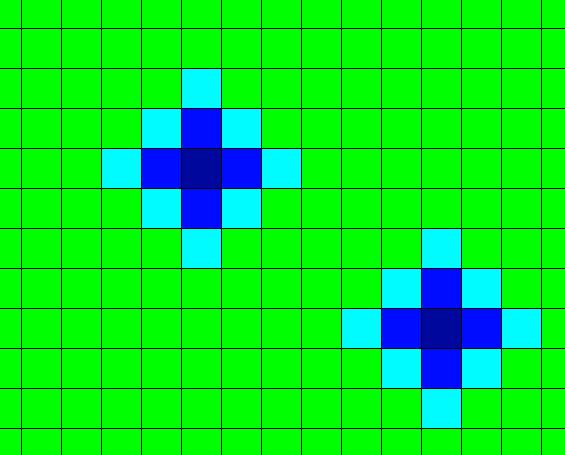
\includegraphics[scale=0.2]{images/Part3RemoveFirstCharge}}
	\end{tabular}
		\caption{Terrain Manipulation Example}
	\end{figure}
	
	\subsubsection{Action-Phase}
	Now we get to the practical part. After planning out the path by deforming the terrain the player now needs to move. Moving along hills makes us sliding and thus gaining or losing speed flexibly. The hill slopes influence our speed. We are equipped with a jetpack to alter our velocity for further increasing or decreasing our speed. The speed helps us getting further. If we are too slow we might lose. So raising the hills must be carefully considered in the first phase.
	There will be further obstacles like turrets that are distributed on the map. The player needs to avoid getting shot.
	\begin{figure}[ht]
		\centering
		\begin{tabular}{cccc}
			\subfloat[Start with no Speed]{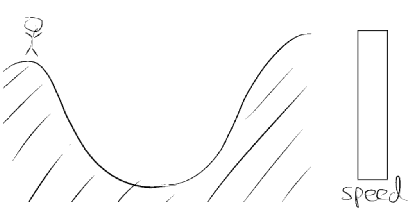
\includegraphics[scale=0.35]{images/StoryboardMovementPart1}}&
			\subfloat[Speed Increase due to Gravity]{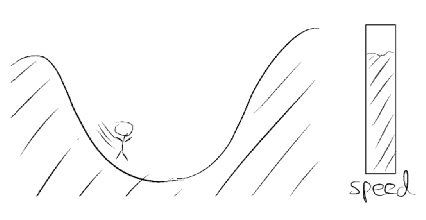
\includegraphics[scale=0.35]{images/StoryboardMovementPart2}}&
			\subfloat[Speed Decrease due to Gravity]{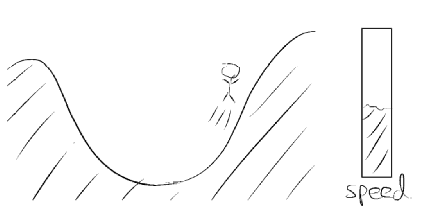
\includegraphics[scale=0.35]{images/StoryboardMovementPart3}}&
			\subfloat[No Speed after short Jetpack Boost]{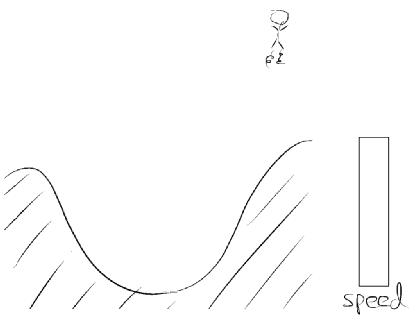
\includegraphics[scale=0.35]{images/StoryboardMovementPart4}}
		\end{tabular}
		\caption{Terrain Manipulation Example}
	\end{figure}
	
	\subsubsection{Terrain}
	From the development point of view the level designer not only creates terrains. The level designer must also define several certain areas that can be deformed by the player which will be discussed in the next section. The terrain looks different in each level. Sometimes we got a grassy landscape, or in other cases more rough plateaus. Some scenarios might be even windy and push the player softly around. At some points there will be water in the map as rivers, ponds or lakes. The fall damage is limited to the player's advantage at this point but on the other hand it slows the player down when he slides on it. If the player's speed is too low one might even dive. Grassy areas cause slight frictions so therefore decelerate the player a little bit. Ice causes no friction and rubble areas have very high friction.
	These areas are firstly flat or already hills or valleys according to the default terrain one gets. The player moves the mouse over the whole terrain in the first gaming phase. Deformable areas will be highlighted by blinking, coloring and or sound effects. Once the player picked an area and clicked on it this area raises up to a hill or lowers down to a valley. The longer one hold the mouse button the more the area gets deformed. And this procedure needs to be done until the player thinks he might be able to reach the goal in the second phase. So the whole process of finding or building the path is like solving a puzzle.
	What is being actually changed is the y-value of the terrain and the radius.
	It is possible to change the terrain several times until the player is ready to try it out. Areas that can not be manipulated will be identifiable as colored districts.
	Then in the next phase the player starts with a default speed value. When he slides along the hill the character we are playing accelerates due to physical laws. These accelerations raise the speed. The gained additional speed is crucial to getting further. Didn't the character gain enough speed the slope of the hill was not well considered first. The other case would be if the character is too fast after passing a hill.
	In the upcoming levels the player will be more and more restricted of deforming the terrain so reaching the goal will be more and more difficult.
	
	\subsubsection{Character}
	The player's character is a guy wearing a jetpack and riding on skis. The character's health will be displayed as a health bar. The health bar changes in several cases. It includes fall-damage that depends on relative vectors of slope normals and the velocity. Also when undergoing explosive damages or getting hit by turrets. There again different types of turrets causing other amounts of damage, like rocket-based, impulse-based and laser-based turrets. It's jetpack can be loaded by collecting fuel packs during the entire level so fuel bars will be also displayed.
	The movements of the character changes as the consistencies of different terrains influence the velocity of the character. More on that on the terrain section.
	According to how much the area the player is sliding on is curved, the player can also slide sideways. Either slightly, fully or also not at all.
	The player won't be able to shoot unless he finds gadgets that allow him to do so.
	The player has not infinite trials to deform the terrain. He has for example 5 charges and thus can make 5 changes on the terrain.
	Also the player can place helpers during the manipulation phase. These helper are mines, fuel tanks or other objects that could help him reach the goal.
	
	\subsubsection{Camera}
	There are two kinds of cameras: Planning Camera and Ingame Camera. The planning camera provides an overview so the player will be able to look down at the whole terrain from the top. Also the camera can be zoomed in and is rotateable so eventually one gets six degrees of freedom to move the camera around.
	The ingame camera can be switched between ego perspective and third person. It depends on the model quality and shall make the gameplay more comfortable for the player.
	
	\subsubsection{Obstacles}
	Depending on the terrain or the whole scenarios, obstacles could be turrets that try to shoot the character. There are different types of turrets causing other amounts of damage, like rocket-based, impulse-based and laser-based turrets. Or just borders or even gates that stay on the player's way. A further classification of obstacle types are natural background obstacles like wind. Windy areas might push the player softly around and of course influence his speed.
	
	\subsubsection{Gadgets}
	The borders from the obstacles-section can also be doors or gates. During the first phase the player should not only concentrate on the goal itself since the straight path to it might not be necessarily the correct one. Possible gadgets are keys that open gates. Further gadgets are grappling hooks to get to platforms that are not reachable otherwise. In the manipulation phase-section was mentioned that the player can place walls to run on. But to be able to do that one needs to collect special boots first which are positioned somewhere in the terrain. This again depends on the terrain consistency. Metallic grounds give metallic walls. In this case the player needs to collect magnetic boots. Each wall type provides running in each direction.
	
	\subsection{Technical Achievement}
	Our focus on technical achievement is the manipulation of the terrain or level in real time by the player to manipulate the speed he is gaining or losing constantly.
	To achieve that from the development point of view we get access to the heightmap and modify it. Then the terrain geometry and respective textures can be updated when the player changes the terrain. Changing is done easily as the ingame tool has very few parameters such as radius, amount and changing the +y-value of the terrain for raising and -y-value for lowering.
	As mentioned at the very beginning of the game description-section modifiable or restricted areas of terrain are highlighted. For example a sound effect starts, the area is colored when hovering the mouse over it or the area blinks.
	
	\newpage
	\subsection{Big Idea Bullseye}
	\begin{figure}[ht]
		\centering
		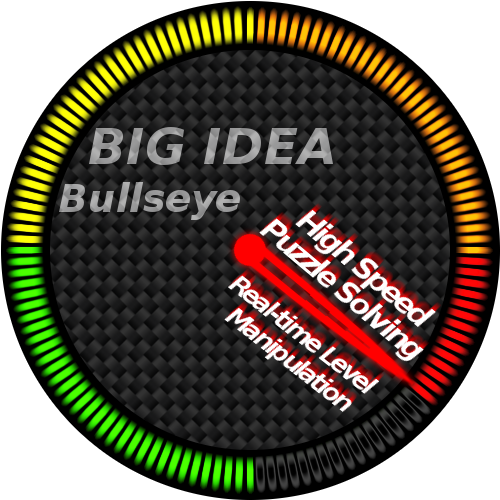
\includegraphics[scale=0.7]{images/bigIdeaBullseye}
		\caption{Big Idea Bullseye Image}
		\label{bigIdeaBullseye}
	\end{figure}
	
	\subsection{Tasks}
	
	\subsubsection{Development Schedule}
	The exploded development schedule for the project can be seen in Figure \ref{developmentSchedule} or in the attached image.
		\begin{figure}[H]
			\centering
			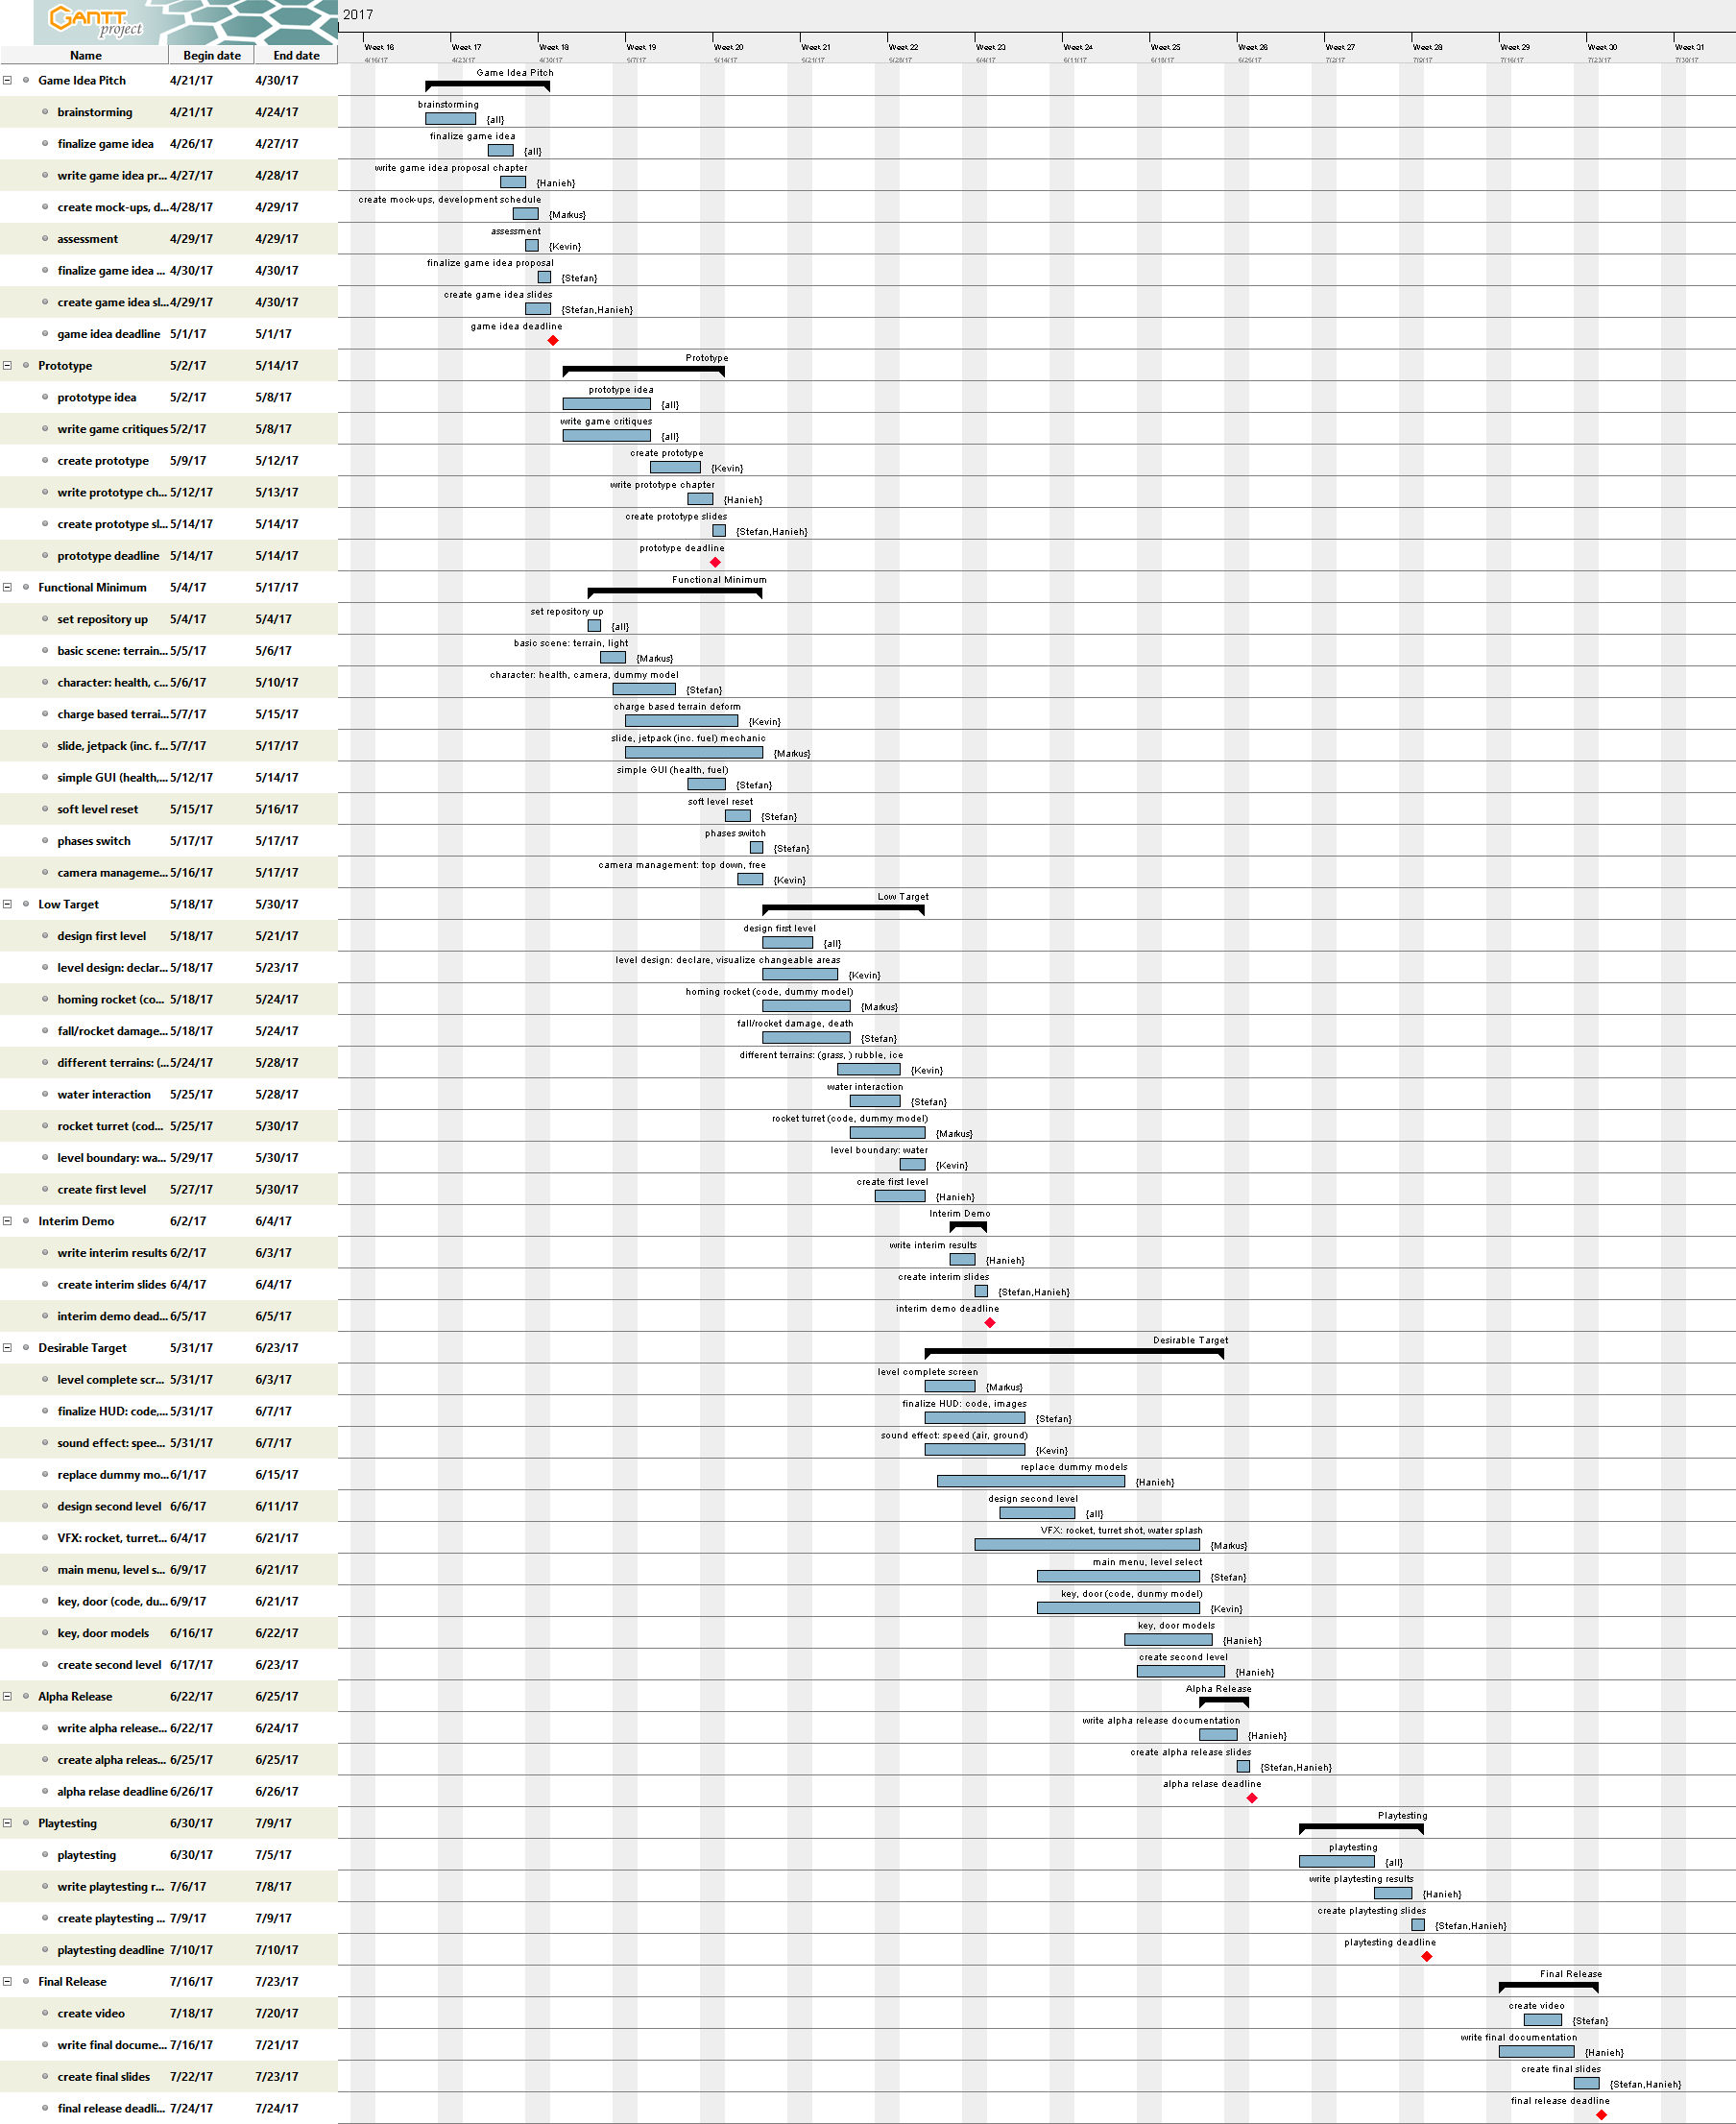
\includegraphics[height=\textheight]{images/GamesLab2017SS}
			\caption{Development Schedule}
			\label{developmentSchedule}
		\end{figure}
		
	\subsubsection{High Target}
	\begin{itemize}
		\setlength\itemsep{0.1pt}
		\item sound effects: rocket, death, goal, taking damage, sliding
		\item time based obstacles
		\item different turrets: impulse, plasma
		\item grappling hook, flying objects
		\item more levels
	\end{itemize}
	
	\subsubsection{Extras}
	\begin{itemize}
		\setlength\itemsep{0.1pt}
		\item background music
		\item level designer for player
		\item target shooting
		\item manipulation of terrain during action phase (slowmotion)
		\item other gadgets
	\end{itemize}
	
	\subsection{Assessment}
	The game is a strategic puzzle game with action elements. The main strength will be the interaction between the manipulation and the action phase. In the manipulation phase you can change the height of several areas of the map in a way that benefits you in the second phase. In the action phase you can slide along hills and use different gadgets to get to your destination and solve the puzzle. The big challenge will be to manipulate the map in a way where you can slide with the right amount of speed to get to your destination.
	This kind of game will most likely appeal to a puzzle games liking or strategic thinking audience. But casual players could also be interested in such a game because of the fast paced action phase.
	An important part will be to make interesting puzzles which will be challenging to solve. So that the player has to think about which terrains to manipulate and how. But also be very careful at which point in time he/she uses the available gadgets.
	
	\newpage
	\newpage
	\section{Game Prototype}
	\subsection{Introduction}
	Our idea is to create a game where the player needs to deform a terrain in order to gain speed due to physical laws. The game consists of two phases: The manipulation and the action phase.
	In the first phase, the manipulation phase, the player has to deform the terrain to his advantage. He can create hills or place gadgets like fuel tanks. When he raises the terrain at a certain point he gets hills. And the hills again provides certain slopes which are important for the next phase. 
	In the action phase the player has to slide along the hills that he has created in the previous phase. The slopes of the hills have an important influence on the speed and cause a momentum that the player needs to reach the goal. If the speed is not high enough a helpful gadget like fuel tanks can help the player to compensate deviations or losses.
	So during manipulation phase the players needs to consider his steps very well and think strategically. And during the action phase his movements are based on physical laws so he needs to slide and move correctly along.
	
	\subsection{Game Rules}
	During the manipulation phase the player can not deform the terrain as much as he wants. He gets a certain amount of charges. E.g. five charges mean, that the player has five possibilities to deform the terrain. 
	Besides the charges he has also a certain amount of fuel tanks that he is allowed to use. For example two fuel tanks simply mean that he can place two fuel tanks all over the terrain except for the restricted areas. Using a fuel tank meant to be able to move about 5 cm in each direction.
	Turning this idea into a prototype we decided to make a sandbox. We crafted a box made out of wood and filled it with sand.
	\begin{figure}[H]
		\centering
		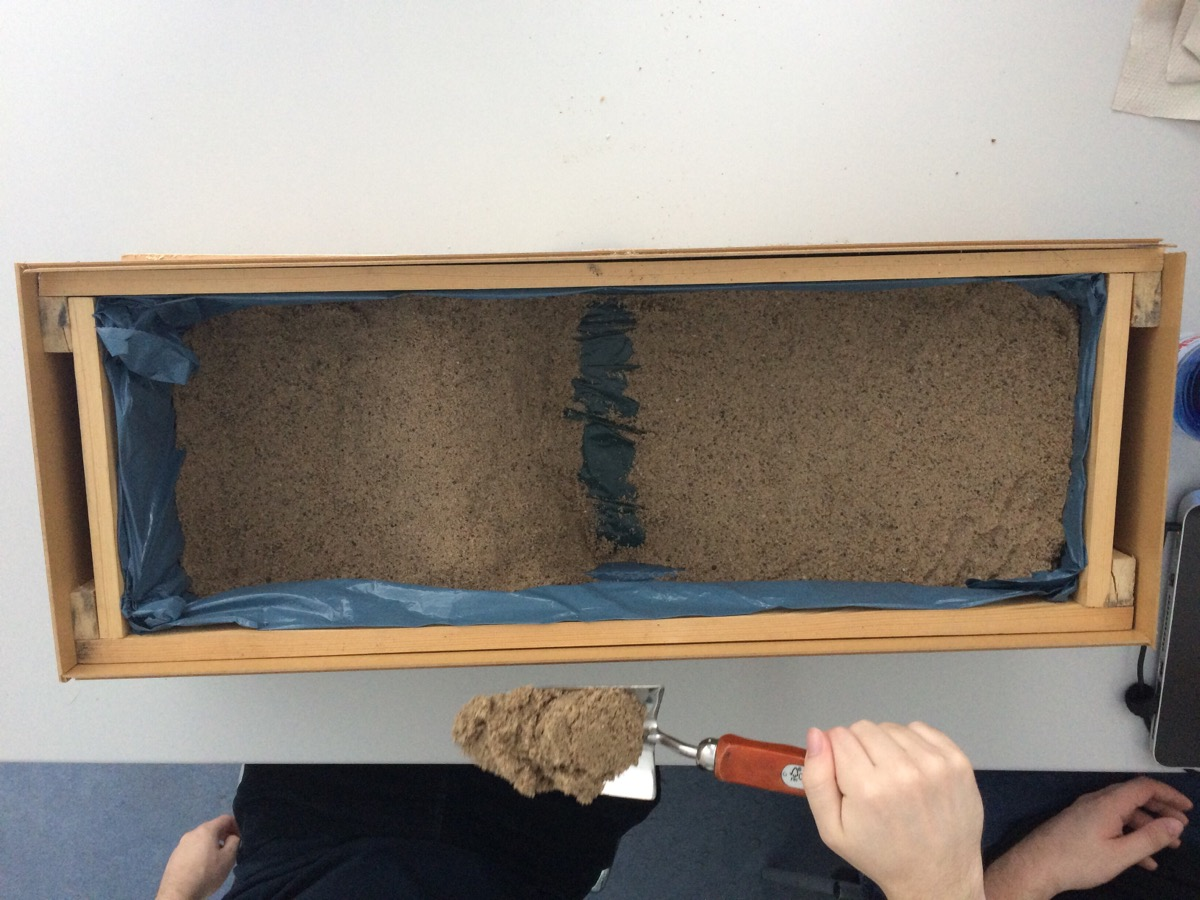
\includegraphics[scale=.2]{images/prototype/prototypeOverview}
		\caption{Prototype Overview}
		\label{prototypeOverview}
	\end{figure}
	During the manipulation phase we shaped the sand and made some hills. For fuel tanks we just cut some papers.
	\begin{figure}[H]
		\centering
		\begin{tabular}{cc}
			\subfloat[Example Hill]{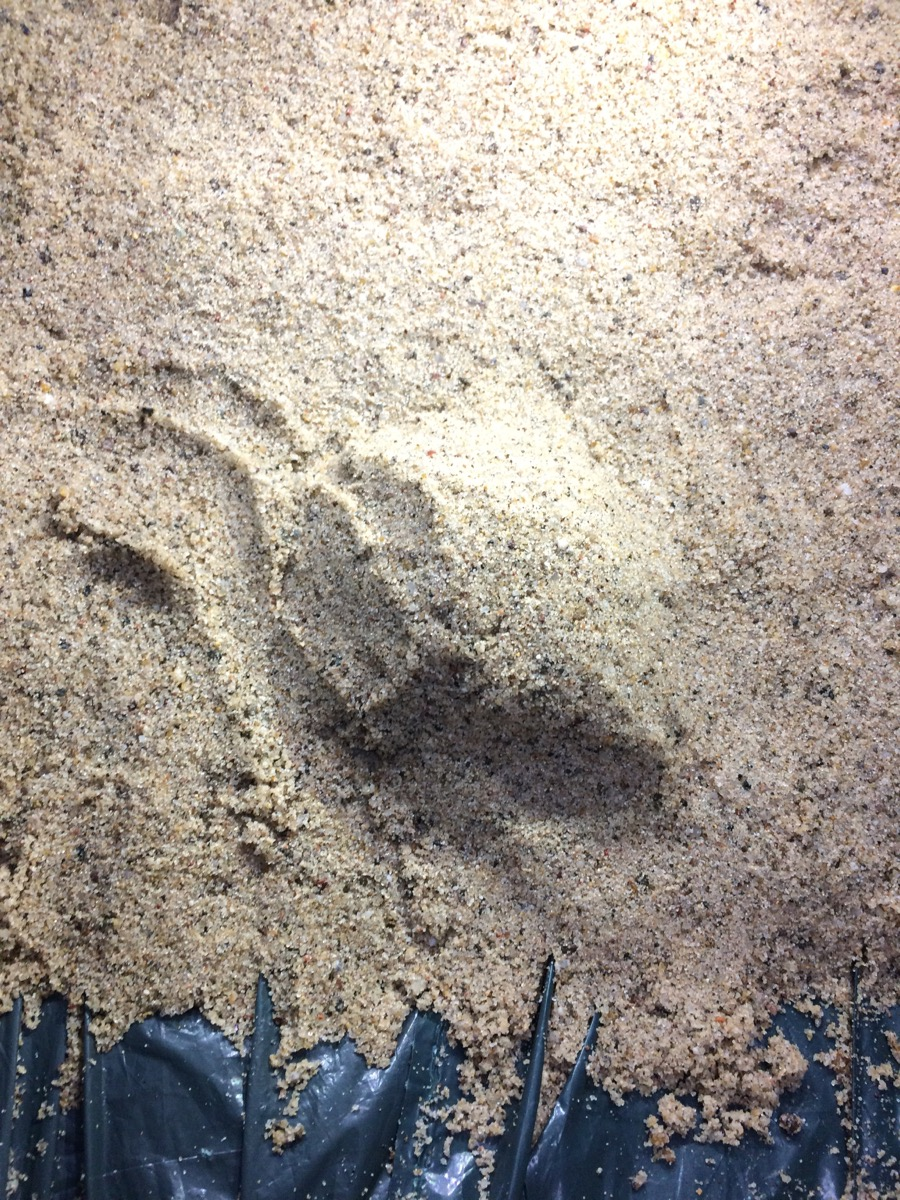
\includegraphics[scale=0.2]{images/prototype/prototypeHill}}&
			\subfloat[Fuel Tanks]{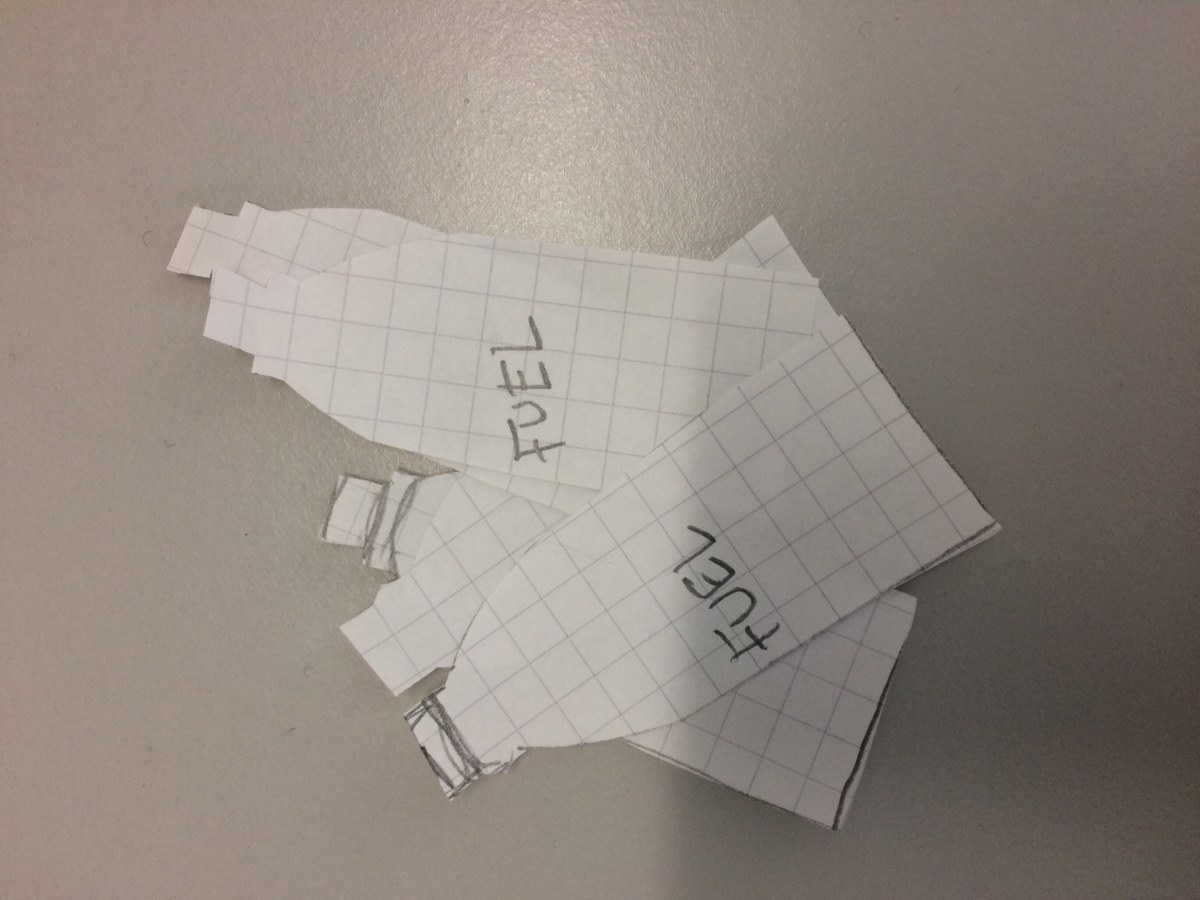
\includegraphics[scale=0.2]{images//prototype/prototypeFuelTanks}}
		\end{tabular}
		\caption{Prototype Explanation}
	\end{figure}
	The character is represented by a marble. In the first step we start at an arbitrary point and then roll down towards the first point that we decided to deform. Sliding along the hill gives us speed to overcome the deadly valley.
	\begin{figure}[H]
		\centering
		\begin{tabular}{ccc}
			\subfloat[Timestep 1]{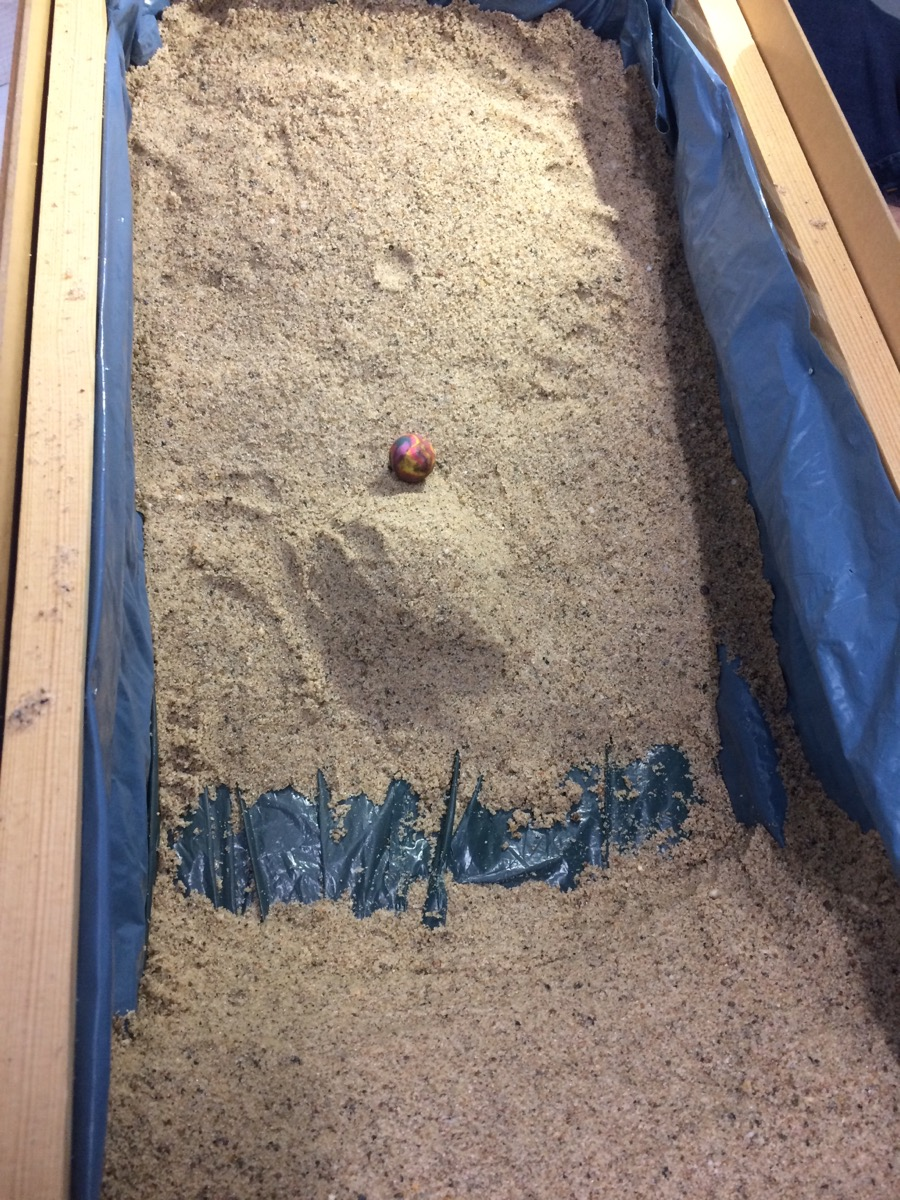
\includegraphics[scale=0.13]{images/prototype/prototypePlaythrough_1_1}}&
			\subfloat[Timestep 2]{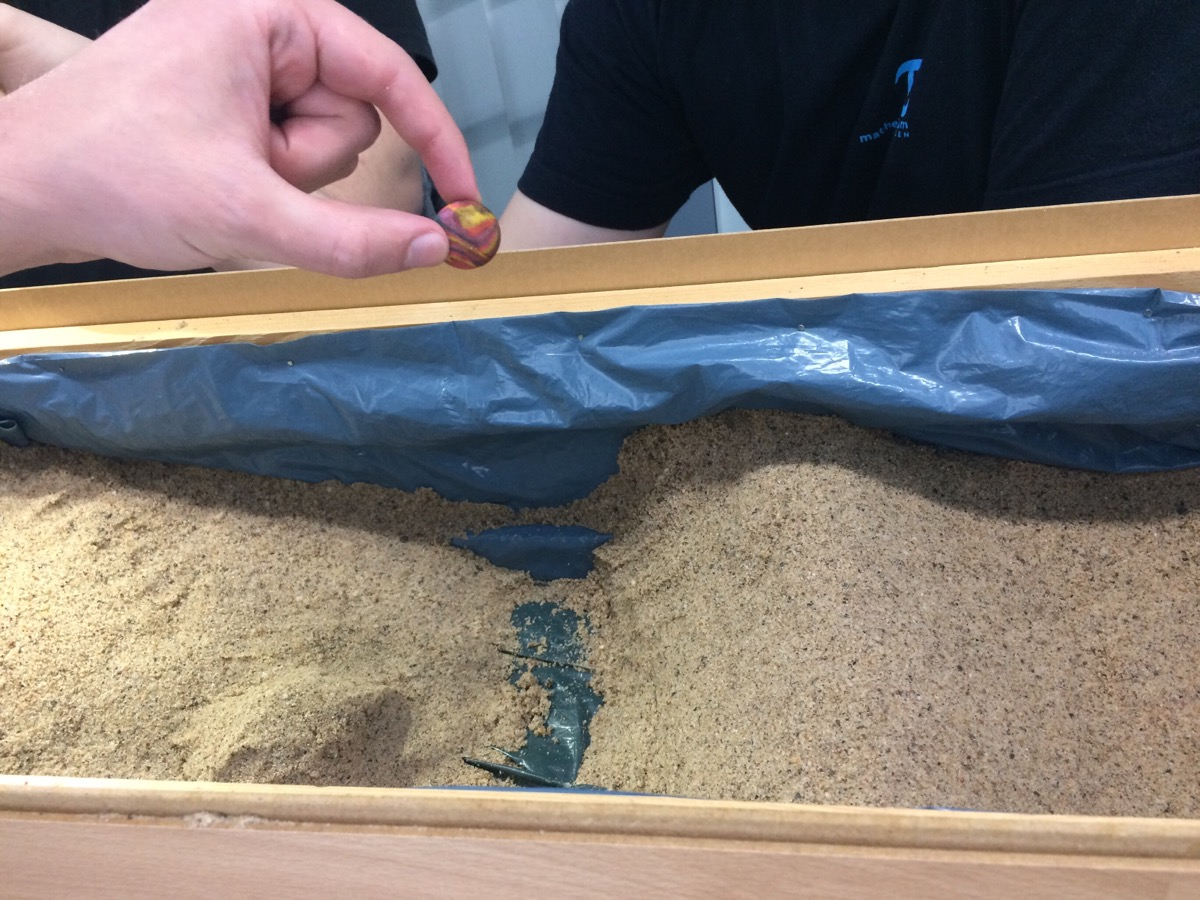
\includegraphics[scale=0.13]{images/prototype/prototypePlaythrough_1_2}}&
			\subfloat[Timestep 3]{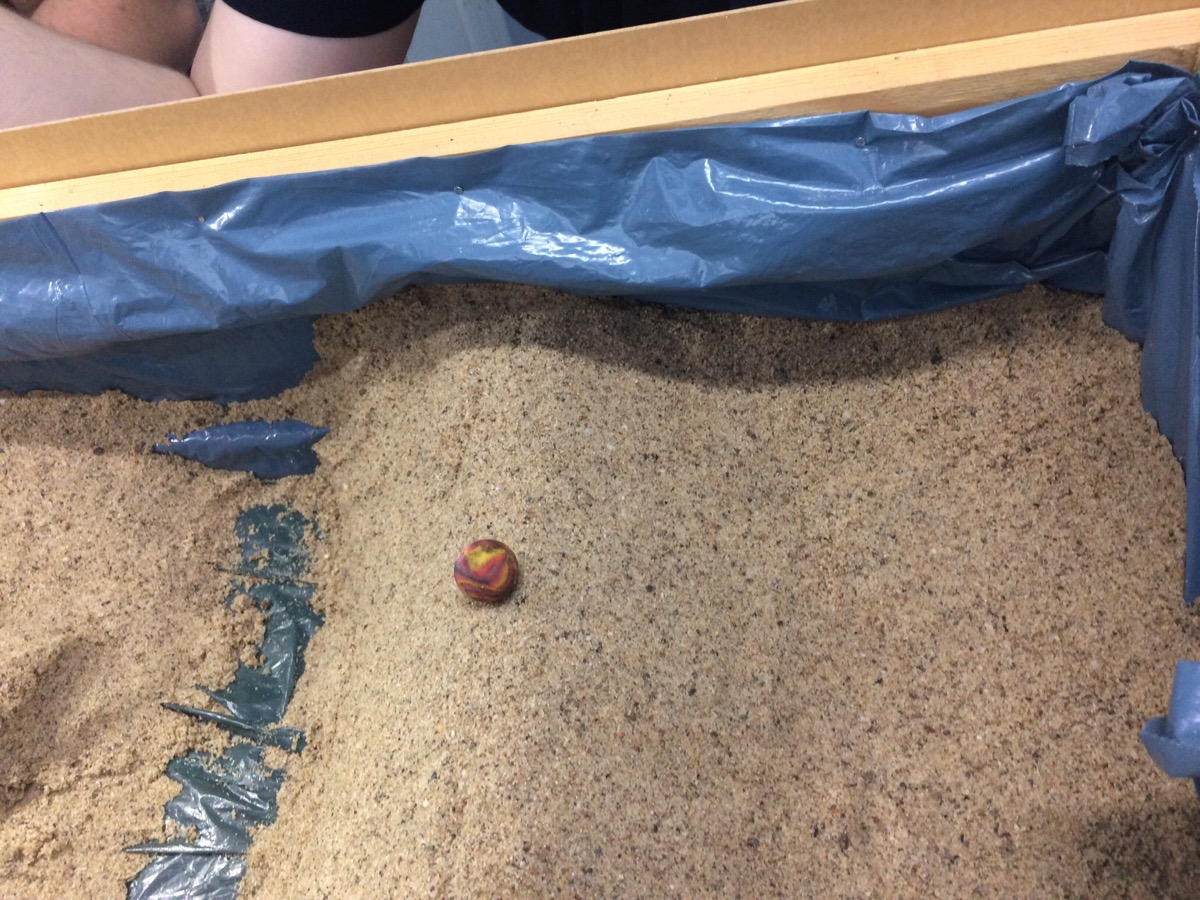
\includegraphics[scale=0.13]{images//prototype/prototypePlaythrough_1_3}}
		\end{tabular}
		\caption{First Level}
	\end{figure}
	It was hard to simulate the acceleration since sand was not an optimal ground due to high friction. But still sand was a good decision when one wanted to deform the terrain.
	
	\subsection{Experience}
	Level design won't be easy since we will need quite a lot time to invent some good levels. It was a challenge to create a puzzle that was fair balanced between easy and hard. One of the remarkable experiences was the fact that the player needed a lot more time to solve the puzzle than we needed to create it. For comparison we needed about five to at most ten minutes to create a simple puzzle. But the player needed about twenty minutes to find a way to reach the goal. This tells us how different the chains of thought between the level designer and the player can be. 
	
	Three of us designed the level while the other person left for a while. One side of the terrain was lower than the other side. Unfortunately this is not identifiable on the pictures. On the higher area we put a wall. Almost one half of the wall soared above the lower area. At this point the player wouldn't be able to jump. The pencil marks the start point and the ball pen marks the goal. 
	\begin{figure}[H]
		\centering
		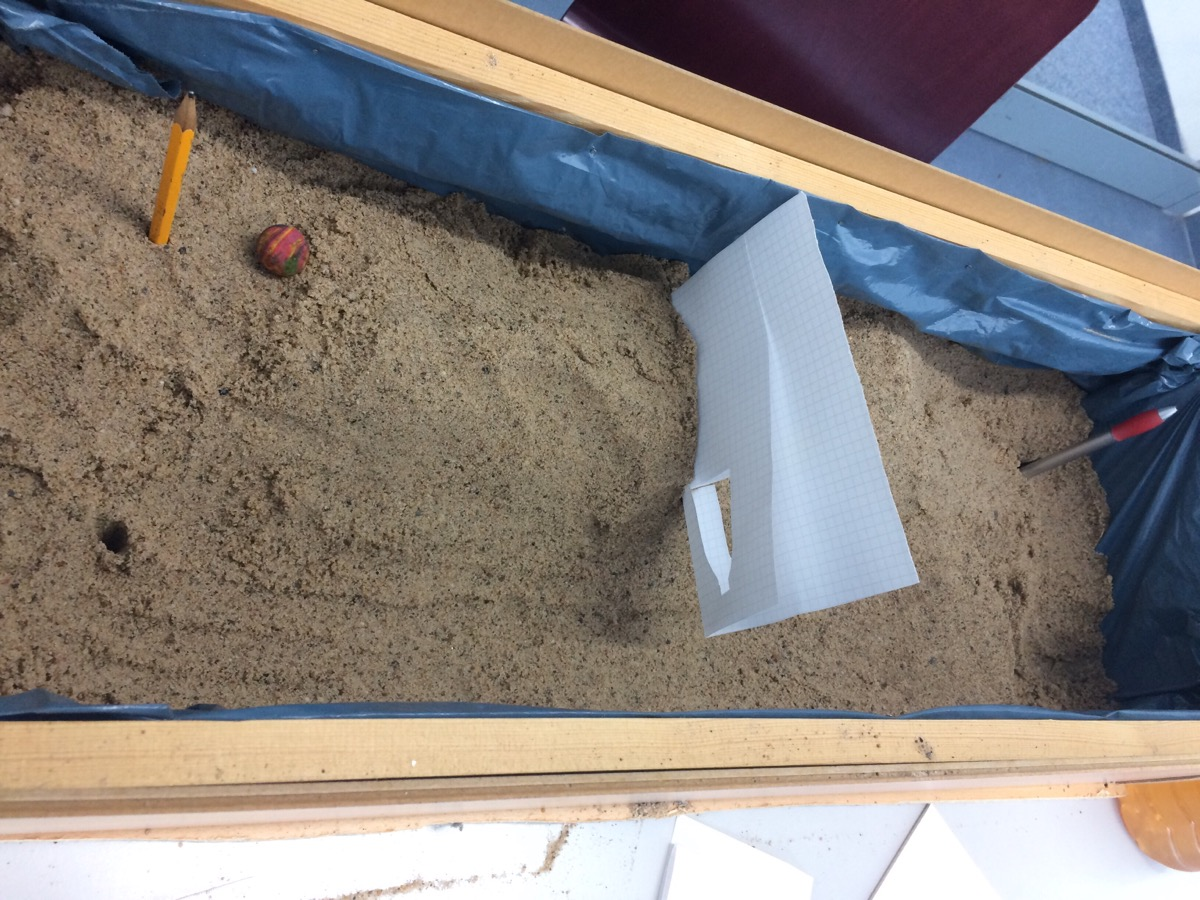
\includegraphics[scale=.2]{images/prototype/prototypeTerrain2}
		\caption{Second Terrain}
	\end{figure}
	Then the player came and started to play. We allowed him to have two charges and one fuel tank. 
	Entering the manipulation phase he firstly placed the fuel tank.
	\begin{figure}[H]
		\centering
		\begin{tabular}{cc}
			\subfloat[Experimenting]{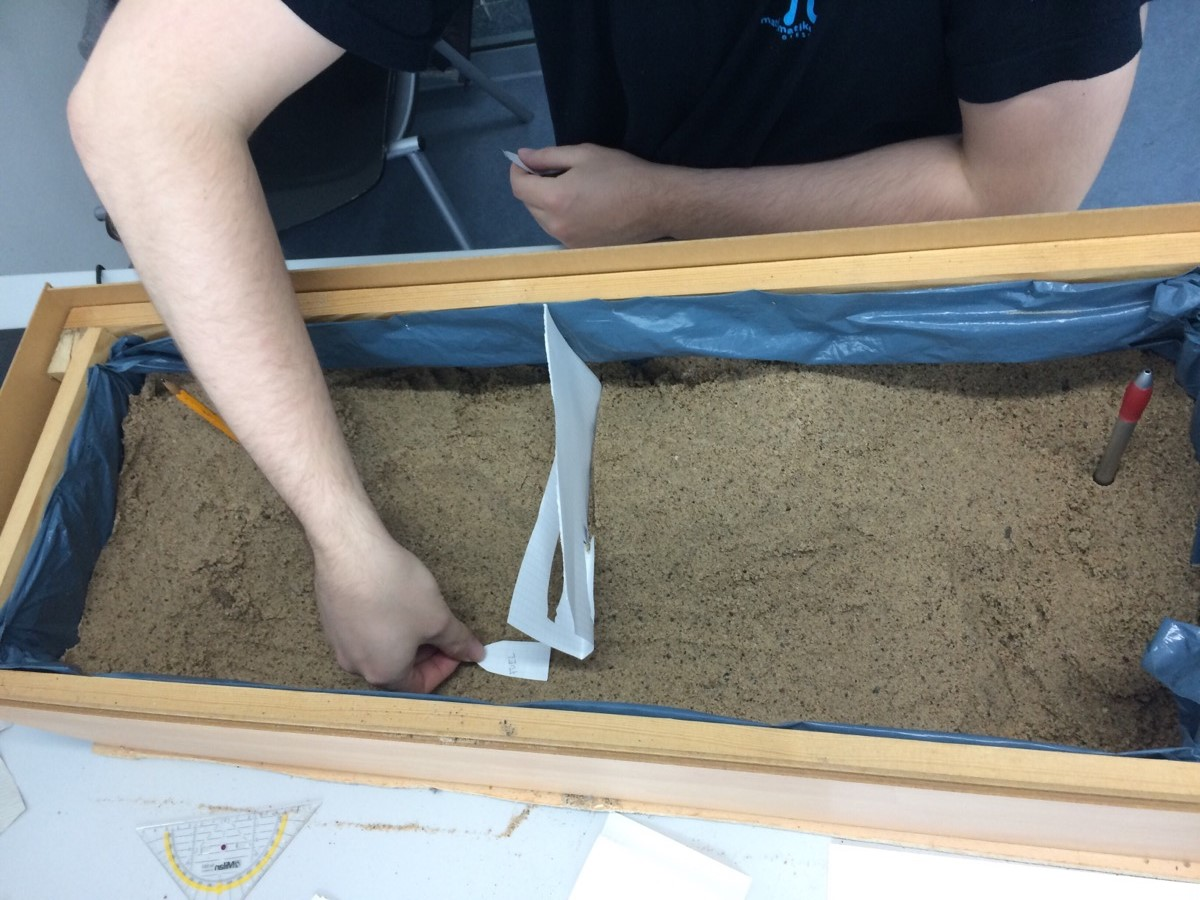
\includegraphics[scale=0.25]{images/prototype/prototypeFuelPlacements1}}&
			\subfloat[Final Location]{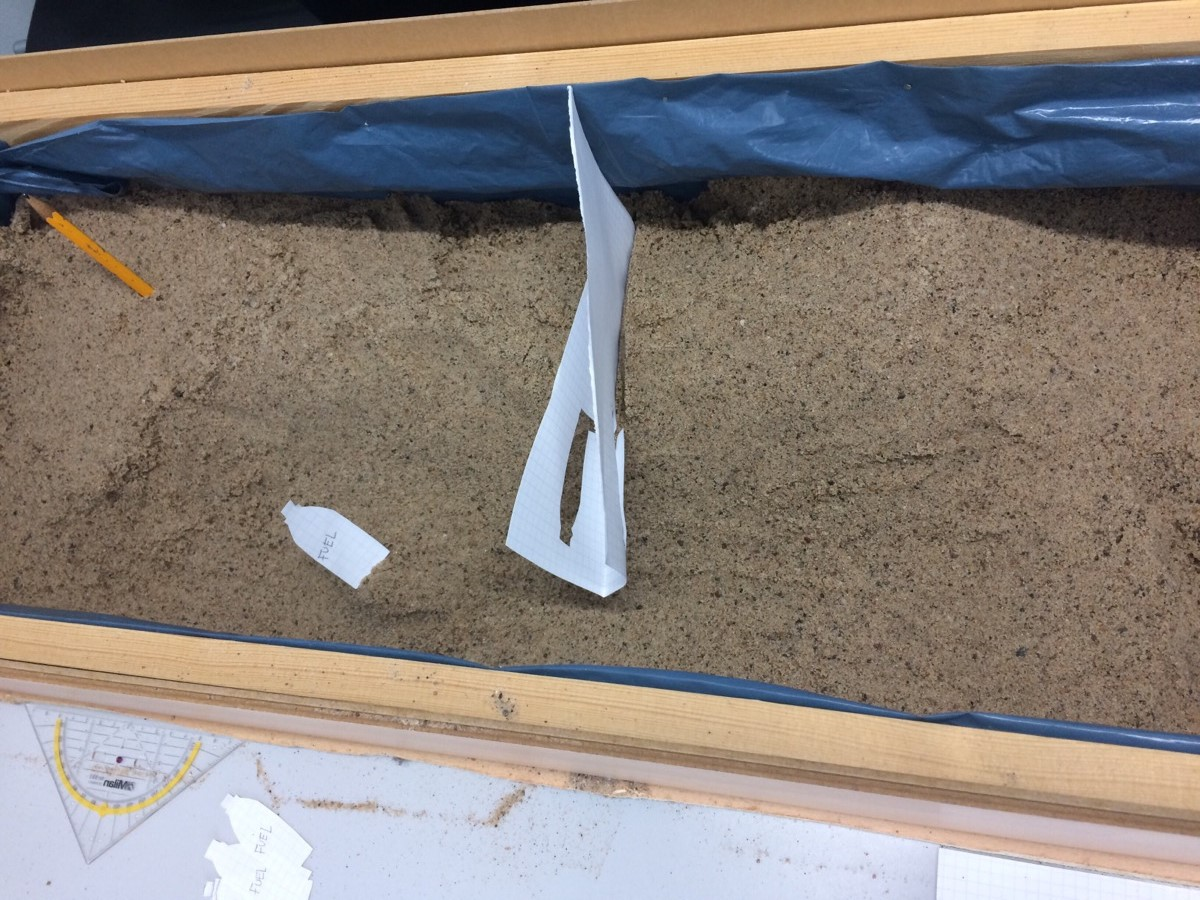
\includegraphics[scale=0.25]{images//prototype/prototypeFuelPlacements2}}
		\end{tabular}
		\caption{Fuel Tank Placement}
	\end{figure}
	Then after some deliberations he picked a spot for the hill. One of us, representing the CPU, built the hill for him.
	\begin{figure}[H]
		\centering
		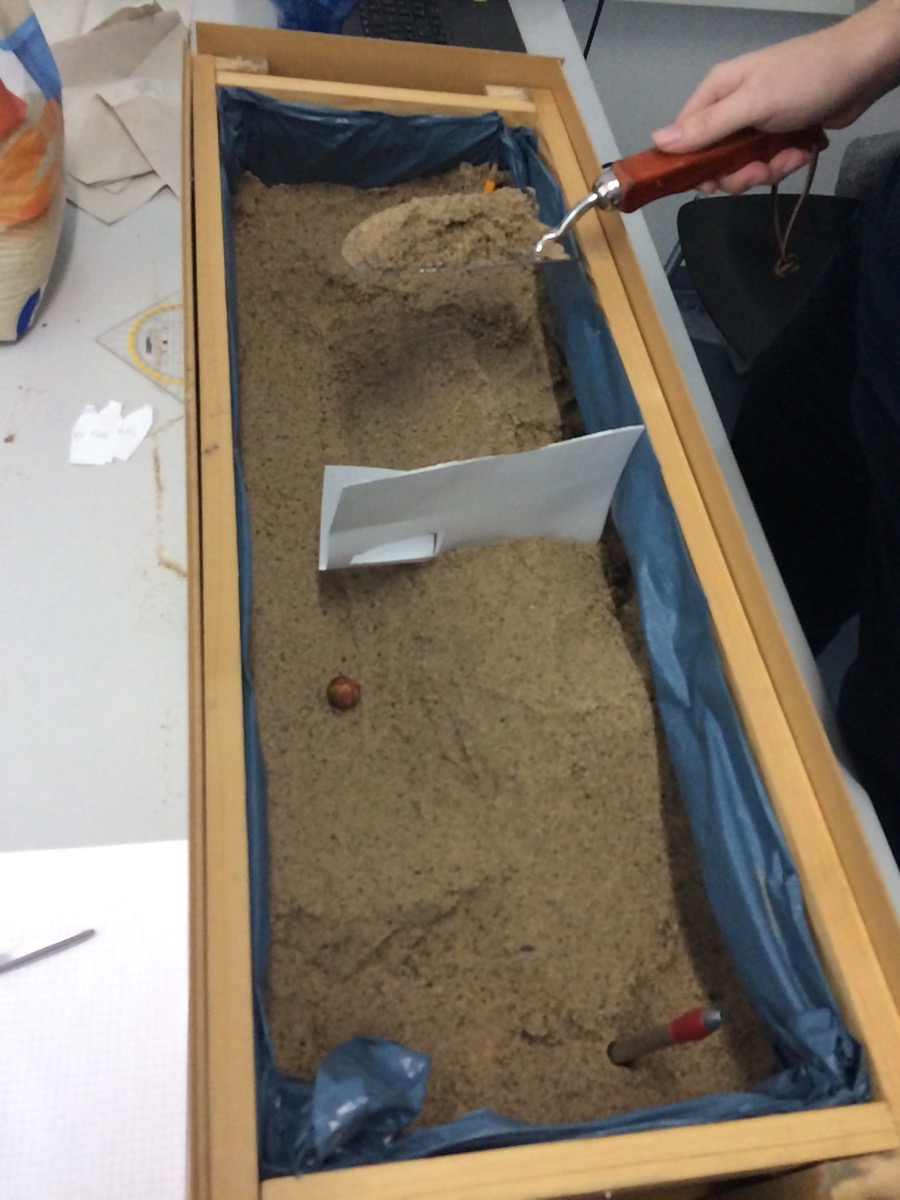
\includegraphics[scale=.2]{images/prototype/prototypeHill1}
		\caption{First Hill}
	\end{figure}
	But the player also decided to raise the same hill once gain because of the idea to gain more speed at the end by sliding along a higher hill.
	\begin{figure}[H]
		\centering
		\begin{tabular}{ccc}
			\subfloat[Step 1]{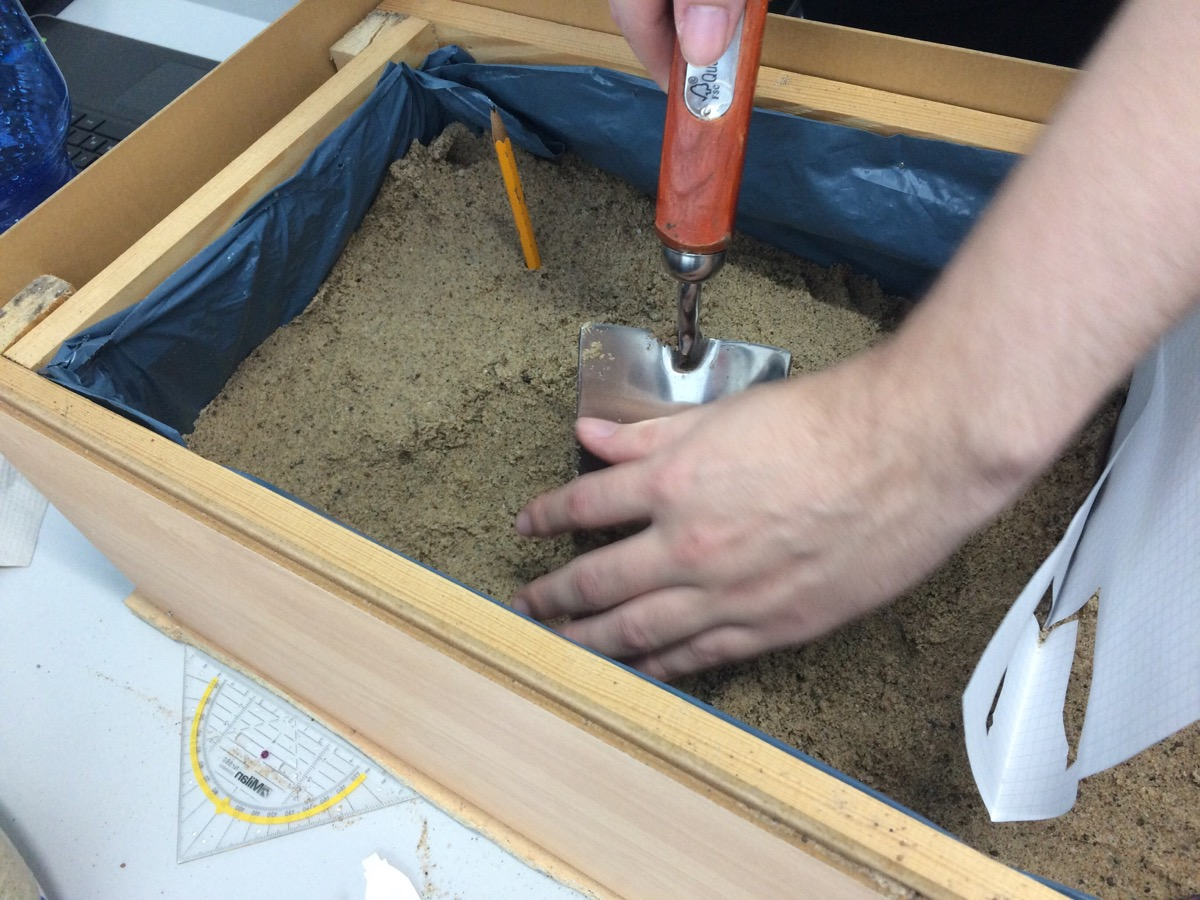
\includegraphics[scale=0.13]{images/prototype/prototypeHill2}}&
			\subfloat[Step 2]{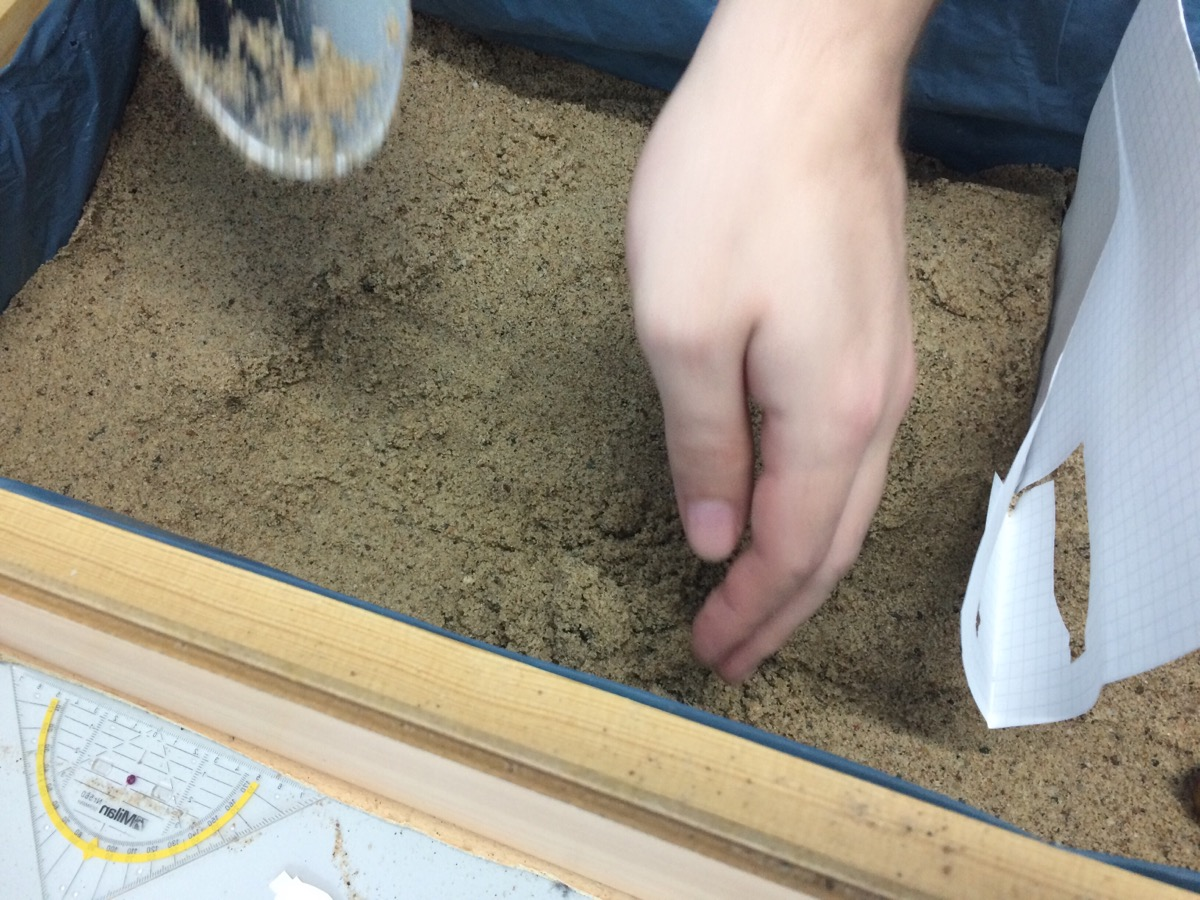
\includegraphics[scale=0.13]{images/prototype/prototypeHill3}}&
			\subfloat[Step 3]{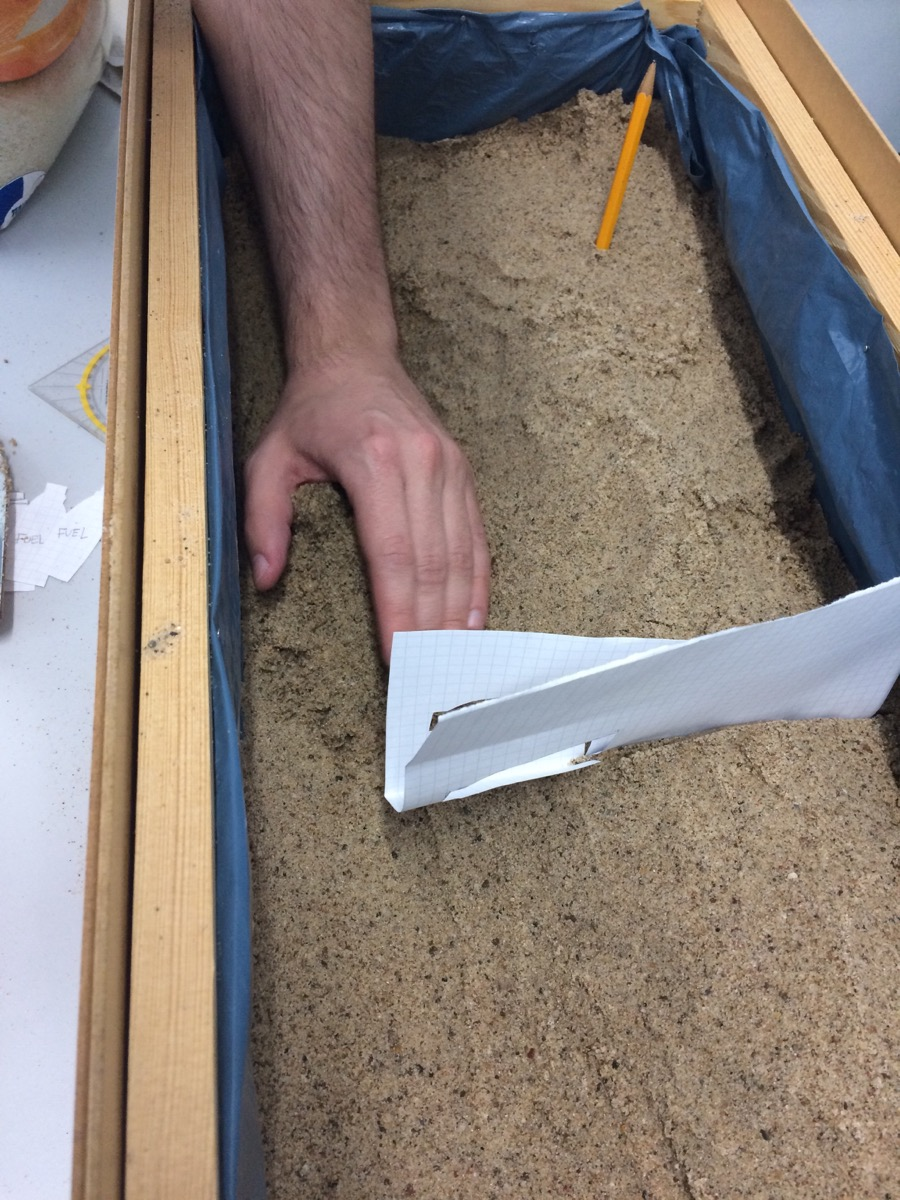
\includegraphics[scale=0.13]{images//prototype/prototypeHill4}}
		\end{tabular}
		\caption{Second Hill}
	\end{figure}
	When he was finished he initialized the action phase. He moved the marble to the fuel tank right onto the double hill. That made him get a high position from where he used the fuel tank. That made him fast enough to slide along the hill where the goal was set.
	\begin{figure}[H]
		\centering
		\begin{tabular}{cccc}
			\subfloat[Timestep 1]{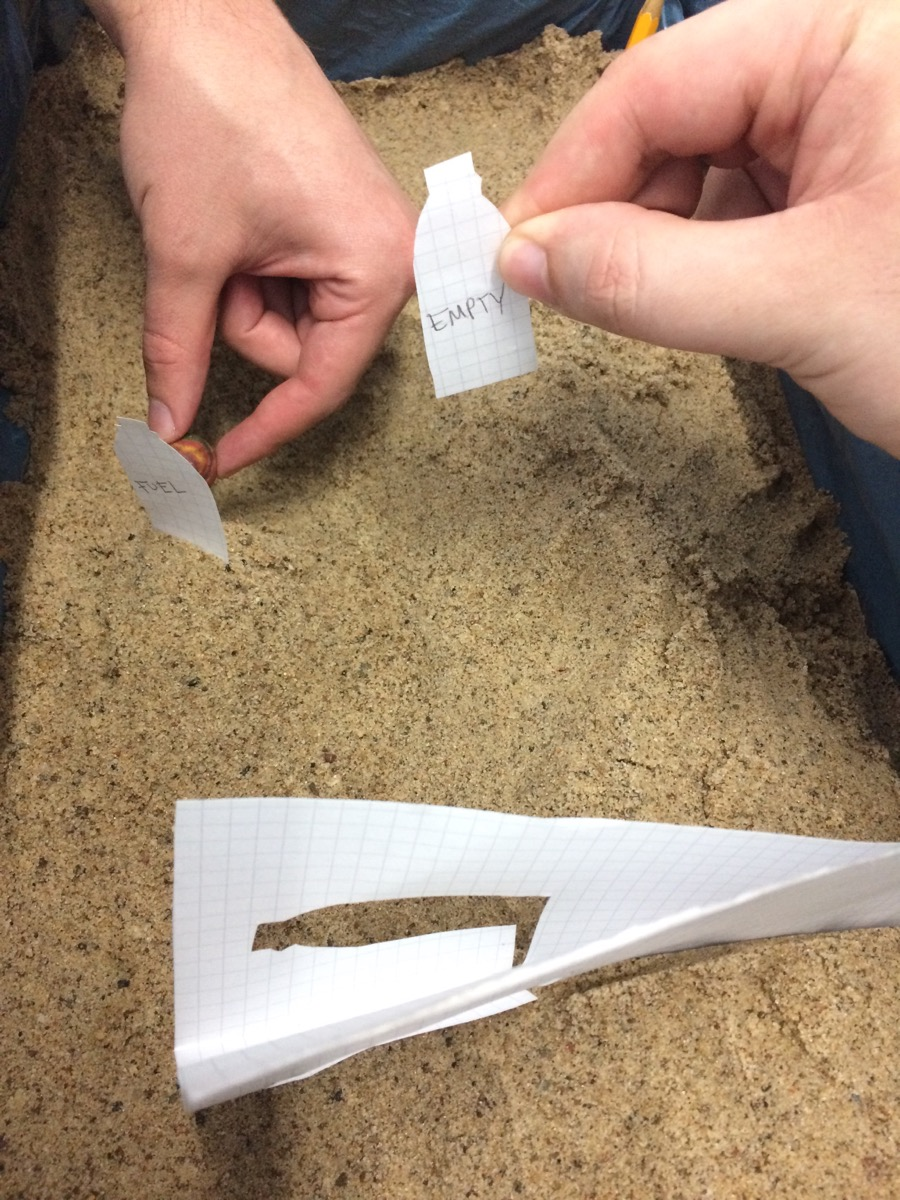
\includegraphics[scale=0.11]{images/prototype/prototypePlaythrough_2_1}}&
			\subfloat[Timestep 2]{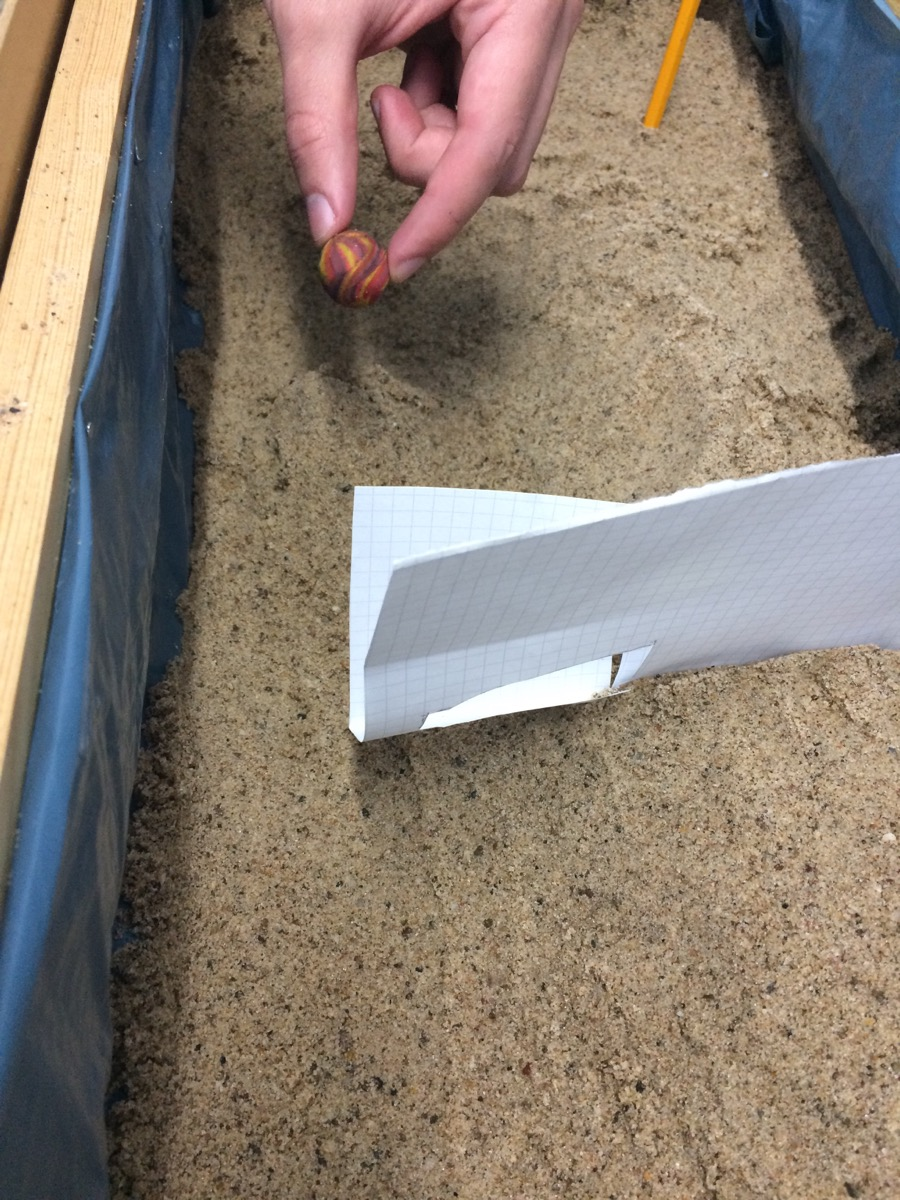
\includegraphics[scale=0.11]{images/prototype/prototypePlaythrough_2_2}}&
			\subfloat[Timestep 3]{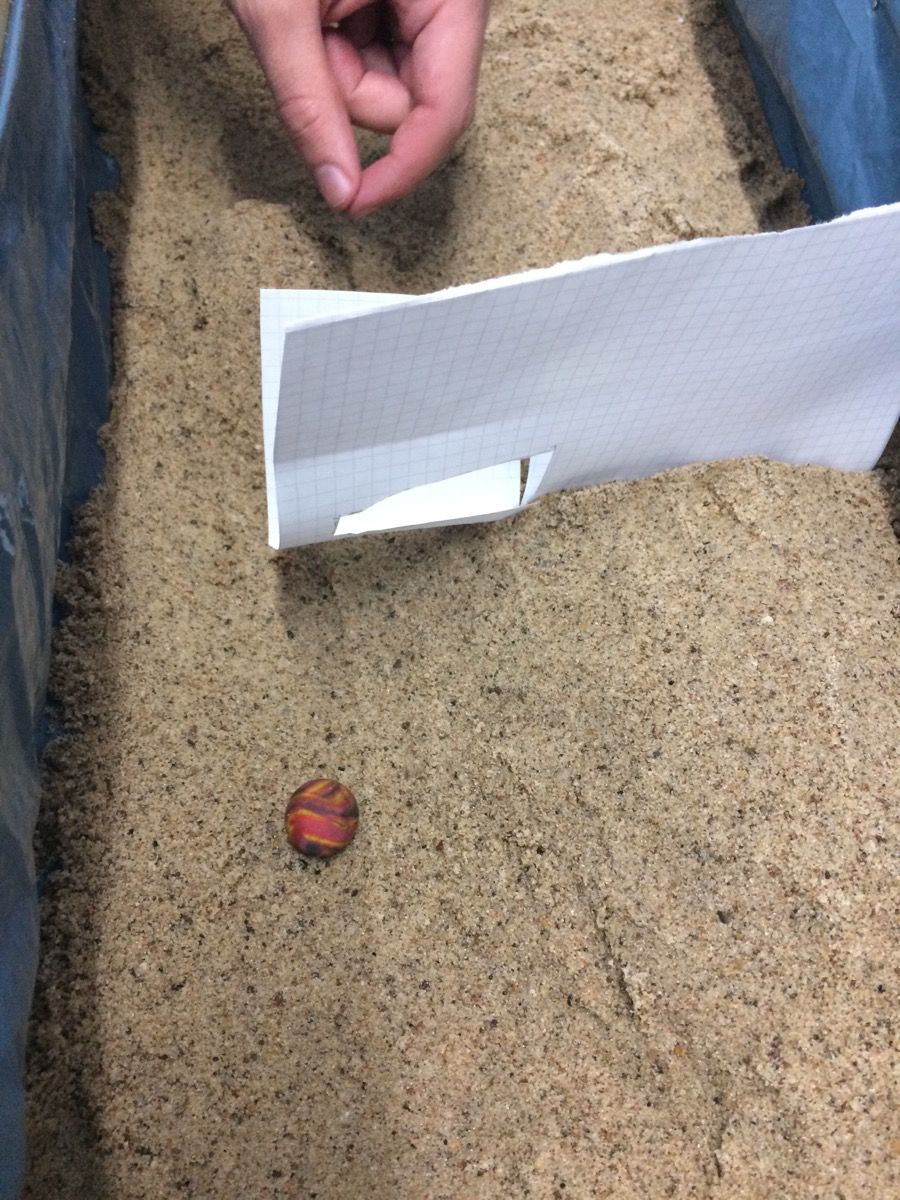
\includegraphics[scale=0.11]{images/prototype/prototypePlaythrough_2_3}}&
			\subfloat[Timestep 4]{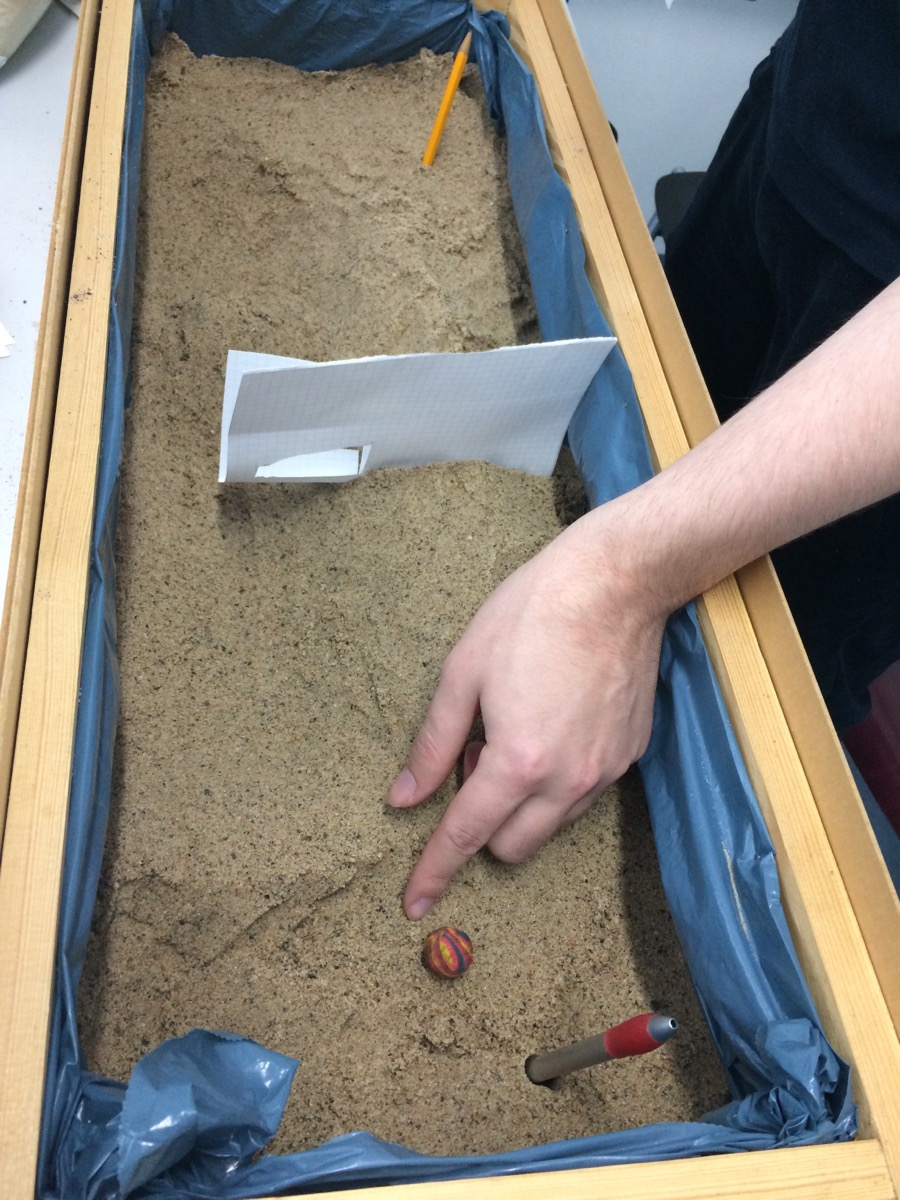
\includegraphics[scale=0.11]{images//prototype/prototypePlaythrough_2_4}}
		\end{tabular}
		\caption{Second Level}
	\end{figure}
	The player needed a few times to solve this problem. We will give the player infinite trials in the future as well.
	
	\subsection{What We Learned}
	Making a prototype means to make the game idea real and touchable. This helps us to get a better imagination and overview of what is in our mind. Deforming the hills with our hand made us better aware of good level designing. By actually touching the world we get a better idea of what could possibly be not logical or what could work. This also has the effect that we can share our imaginations better with other group members since everyone can see what is in our mind. This works better than just talking to the others. And during the discussion everyone can interact with one's imagination by touching our thoughts.
	
	And as already mentioned in the experience-section a further fact that we have learned is that the player needed a lot more time to solve the puzzle than we needed to create it. Having realized this time difference will help us to prevent avoidable mistakes.
	
	\subsection{Critiques}
	The manipulation of the terrain and also the level design will be our main focus of the game, because of the experiences we gathered from the prototype phase and also because it was very well received in the critiques.
	
	Many asked to merge the terrain manipulation into the action phase, but we will still keep it separated. Because it doesn't serve well to the whole puzzle idea and it would be more of an action game. Also it would make the terrain manipulation and the level design much more complicated.
	
	The idea of dynamic terrain is already in the making in the form of dynamic rivers/lakes. But it, along with turret destruction, will be a high target goal.
	
	A sandbox mode was asked, and we will make it in the form of a level editor, but it is set as an extra target.
	
	We will still keep a health bar, because that way we can make more turrets, also the player is able to make some mistakes without dying straight away.
	
	\newpage
	\section{Interims Report}
	\subsection{Functional Minimum}
	\label{sec:functionalMinimum}
	The focus of our functional minimum milestone was mainly on the most basic gameplay mechanics of our game and essential features that are need for it to be called a game. This meant both phases needed to be implemented, the Manipulation- as well as the Action-Phase. The Manipulation-Phase consisted of a controllable, floating top-down camera and the actual manipulation of our terrain. The Action-Phase contained the sliding movement and jetpack mechanic. Another very basic feature was some kind of user interface, which was realized by some text with numbers.
	
	\subsubsection{Basic Character Implementation}
	For both the functional minimum, as well as the low target, the character was represented by a capsule model which was provided by Unity itself. This enabled collision detection and shadow casting and will be easily replaceable with a real and animated model in the desired target. Also part of the basic character was a first person camera, which was a breeze to implement. Another essential aspect of the character script was handling keyboard and mouse input from the player. The basic control scheme is using the mouse to look around in first- and third person view, pressing “WASD” for slightly moving on the ground and in the air, holding down the spacebar to activate the jetpack and pressing enter to switch between both phases.
	
	\subsubsection{User Interface}
	As mentioned in Section \ref{sec:functionalMinimum} the user interface only consists of text with numbers for now (see figure \ref{fig:screenshot}). The displayed information changes depending on the current phase the player is in. In the Manipulation-Phase he can see the amount of charges he has left and in the Action-Phase he can see his current health and remaining fuel.
	\begin{figure}
		%\centering
		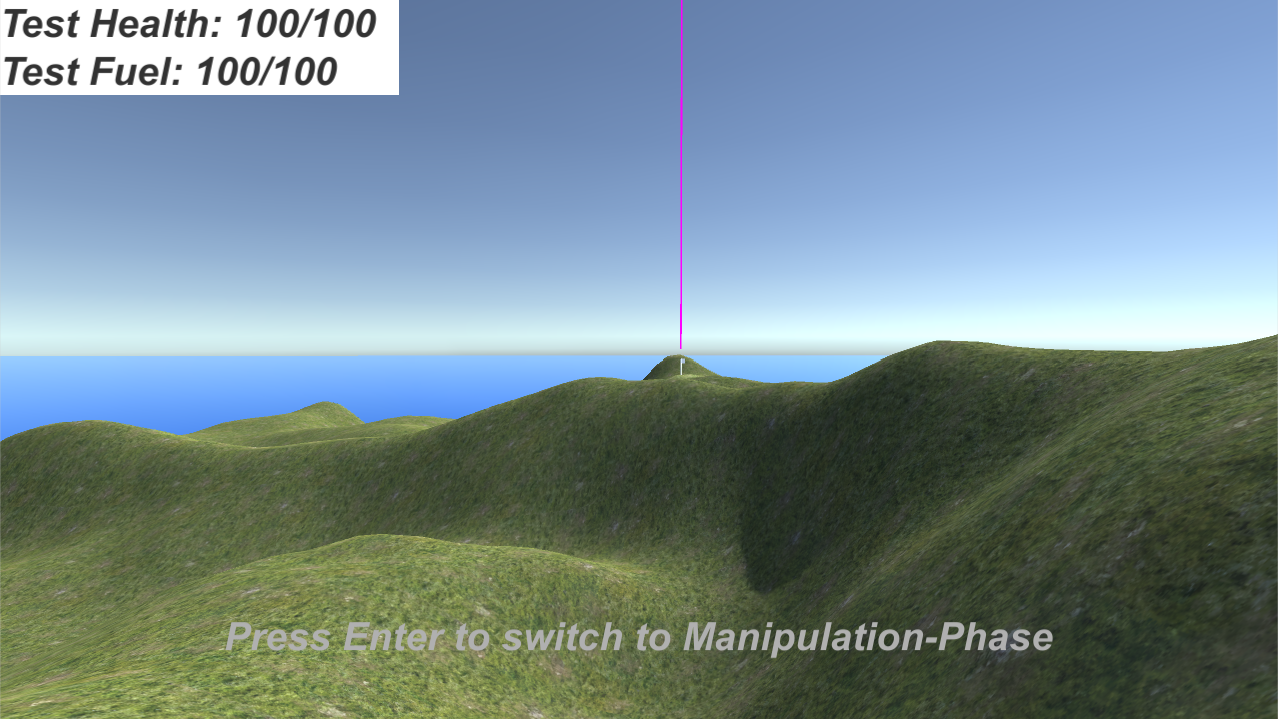
\includegraphics[width=\textwidth]{images/interim/screenshot}
		\caption{Ingame screenshot with UI from Functional Minimum}
		\label{fig:screenshot}
	\end{figure}
	
	\subsubsection{Character Movement}
	Our target for the Functional Minimum was implementing the slide and jet-pack mechanics. The CharacterMovement script handles gravity, velocity slope interactions and is open for other external forces. The Jetpack script receives state messages from the Character script. As long as enough fuel is available and the script is in an "on" state the CharacterMovement script receives an upward motion. Since the basic character and the character movement implementation was split between two different persons, we used multiple interfaces in order to render a smooth development phase possible.
	The CharacterMovement script contains already important parts for the interaction with different terrains planned for the Desirable Target.
	
	\subsubsection{Terrain Manipulation}
	The goal of the manipulation phase was that the player can manipulate the terrain in a way that he/she can raise or lower the terrain at a certain predetermined degree. The player can manipulate the terrain only in the manipulation phase and raises the terrain with a left click, and lowers it with a right click. The manipulation is still not as smooth as it should be and can result in a steeper hill than we would like. But the parameters for the intensity of the manipulation will still need to be checked and adjusted to achieve a balanced gameplay experience. The camera movement was quick and easy to implement. The option to regain charges if the player lowers an already heightened area, is more work than expected and has still to be implemented. An interesting discovery was, that unity saves the changes in the terrain instantly and permanently. To prevent this we must store the unmodified terrain and then use it to reset the terrain after a level is completed or aborted to its original state.
	
	
	\subsection{Low Target}
	Having finished the core mechanics of our game in the Functional Minimum milestone, the focus of the Low Target milestone was making our game actually playable by designing the first level (in this case even the first few levels) and implementing some important gameplay elements like the first turret. Even though the plan was to implement further features regarding the terrain (marking areas as not manipulatable, different surfaces), we did not have enough time for them due to the fact that the implementation of the manipulation itself took longer than expected.
	
	\subsubsection{Level Design}
	The process of designing our first level was iterative and consisted of multiple steps. First we discussed on how and when all our gameplay mechanics should be introduced to the player. We decided that the first two levels are meant as tutorials, where the first only contained sliding and jetpack use and the second one introduced the terrain manipulation in combination with the movement learned before. The next step was that each of our team members designed a level and we voted on the best ones. After that we made minor changes to the selected levels and integrated them into our game.
	
	\subsubsection{Homing Rocket (Turret)}
	The initial design for the homing rocket envisaged a projectile flying at a certain distance over the ground following the player till either a self-destruction timer triggers or its target. However, always keeping distance to the terrain proved to be more difficult than anticipated. Because of a lack of time the rocket design transformed to a simpler design: It just follows the player and explodes when it collides with the ground.
	Since rockets are triggered whenever the player is too close to a turret, an initial velocity ramp up phase is implemented. This prevents a frustrating experience for the player where has no time to dodge the head-on incoming rocket. The acceleration curve is easily adjusted since it is based on Unity's in-built AnimationCurve.
	
	\subsection{Desirable Target}
	
	\subsubsection{Modeling and Arts}
	We are now in the Low Target. The models are needed for the desirable target but I started with them now. 
	
	For modeling I use Blender. I started with modeling two different defense towers. As a reference image I used a typical turbolaser tower from Star Wars.
	One has dual laser guns shooting two lasers at the same time. The other has got one gun shooting rockets. The are suppose to follow the character later on where the dual lasers are shot straight to an old position of the character. With old I mean a few milliseconds after the new position since the character is moving all the time. But the dual laser tower shoots lasers every third seconds so the character has got a chance to avoid a blow. The rockets are shot every 5 or 10 seconds.
	
	The tower, the head (with the wheels) and the guns are all separated meshes.
	
	The lasers are simple stretched capsules also made with Blender like the rockets.
	
	\begin{figure}[H]
		\centering
		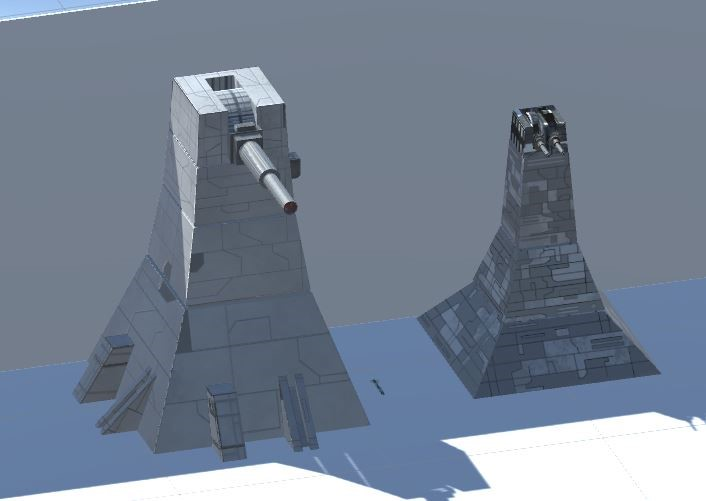
\includegraphics[scale=0.6]{images//interim/turrets}
		\caption{Rocket- and Laser-turret models}
	\end{figure}
	
	\begin{figure}[H]
		\centering
		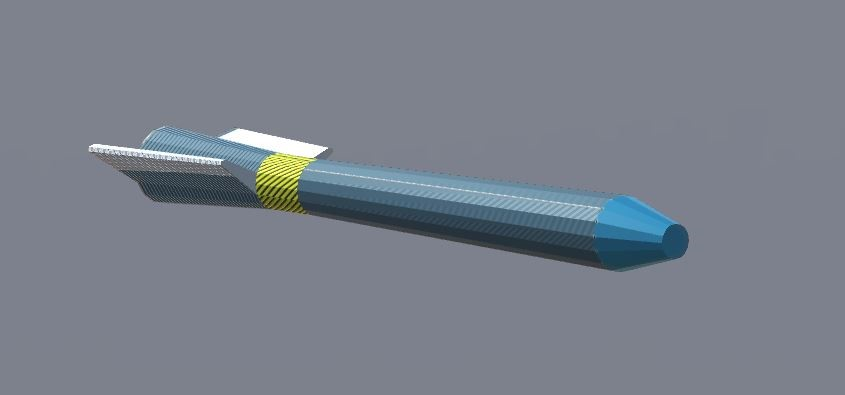
\includegraphics[scale=0.5]{images//interim/rocket}
		\caption{Rocket model}
	\end{figure}
	
	During the cooldown the head of the towers aim the character by moving their heads around the z-axis. At the same time the guns aiming the character rotate planar around the x to y-axis. The guns are attached to the heads. Once the guns shoot they undergo a kickback. The rotations are calculated via scripting using C\# in Unity. The kickback is a simple animation also done in Unity where the gun just go a bit backwards within a very short amount of time to make the kickback fast and then go more slowly to the initial position within a longer amount of time. This is still in process.
	
	The most difficult part is to let the gun rotate around the x and y-axis correctly. The guns are children of the heads so the rotate along the z-axis correctly. But the guns are also attached to a gameObject that is used as a reference point. This game object is placed somewhere under the gun. And if it rotates, the guns rotate around the gameObject to let the player think the gun move along the wheels. Correct setting up this game object as a parent and scripting this special behavior takes the most time.
	
	The textures were made with Gimp where I imported the UV-layout of the guns and drew some lines and dirt effects onto the texture patches. Having done that I created a heightmap and a normal map also with Gimp. These textures are put on the standard shader that is provided by Unity and then applied onto the towers.
	
	Then I modeled the character. I started with helmet and went down to the hands and feet. As a reference image I used a stormtrooper from Star Wars. Then I modeled the jetpack that will be attached to the character as a separate mesh. The visor is a separate mesh too since the material of it will get a glowing effect in the future.
	
	\begin{figure}[H]
		\centering
		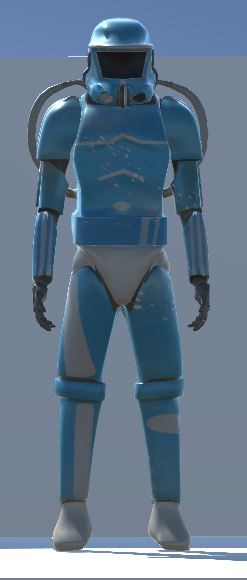
\includegraphics[scale=0.9]{images//interim/character}
		\caption{Character model}
	\end{figure}
	
	The first version of the mesh had more than 50000 triangle. I used the decimated modifier that is provided in Blender to get around 13000 triangles in total. Having a high poly version in the first place makes it easier to model the character.
	It was the first time for me to create a texture of characters. I used to use the "Smart Projecting"-function to unfold a mesh. For this function one does not need to mark seams so it is good for towers for example. At least it is easier for me. But one won't get around of marking seams when texturing a mesh like character. I went through some tutorials and then could create a good UV-layout. I painted it with Gimp then.
	
	In Unity I used again the standard shader with no further special effects to render the textures.
	
	The next new and still a bit difficult part is the animation of the character. I do this also for the first time. I animated all states the character can enter in Blender. Then I imported it in Unity.
	First I got the issue that the each bodypart moved alone without having an effect on the adjacent body parts. This caused the mesh to stretch its neighbors and it looked really bad. This is still in process.
	
	\subsection{Additional Project}
	This section contains a project that can not be classified into one of the layers since it reaches across multiples because of its scope.
	
	\subsubsection{Terrain River}
	The real time river simulation is only dependent on the heightmap of the terrain. It creates rivers by following the path of least resistance till it hits a local minima. Lakes, on the other hand, are created through the filling of a sink. These two phases alternate until a certain min height is reached ($\equalhat$ sea level). 
	The original idea for the path of the river included calculating the current velocity of the stream.  However, this increased the complexity of the algorithm by a large margin and was therefore scrapped. 
	Figure \ref{fig:river1} shows the result of a simulation. In Figure \ref{fig:river2} the player created a dam and rerouted the path of the river.
	
	\begin{figure}[H]
		\centering
		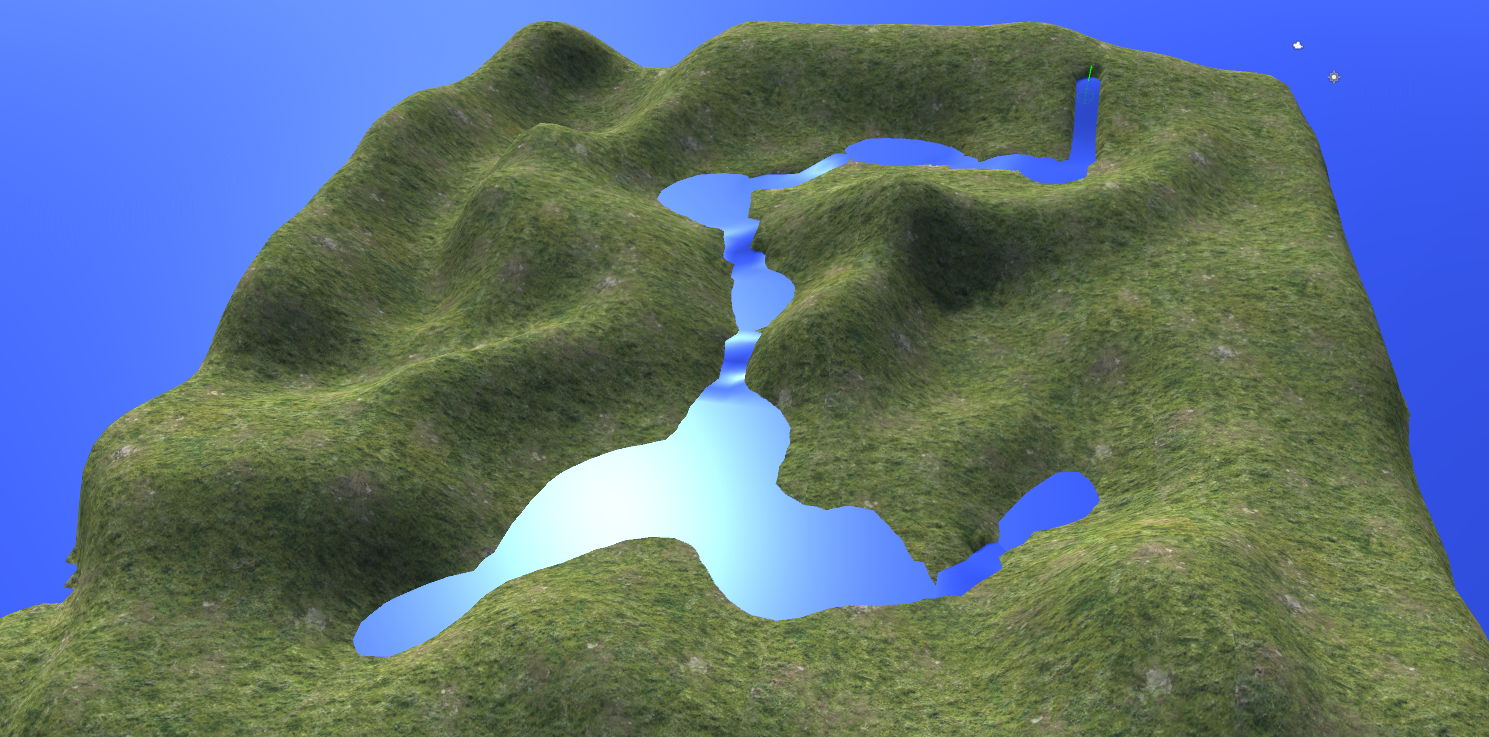
\includegraphics[width=\textwidth]{images//interim/river1}
		\caption{Terrain river without manipulation}
		\label{fig:river1}
	\end{figure}
	
	\begin{figure}[H]
		\centering
		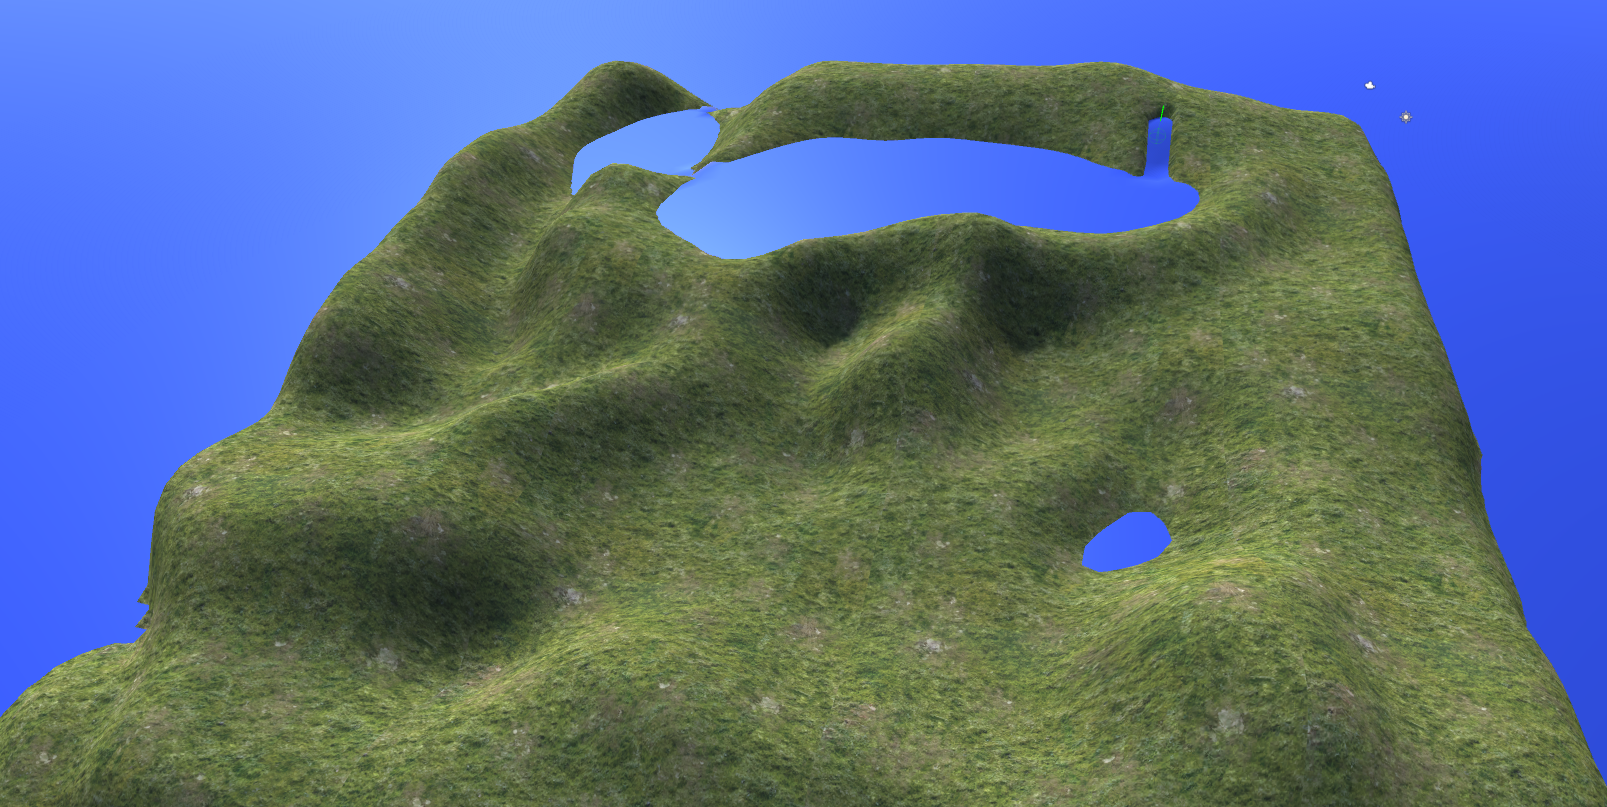
\includegraphics[width=\textwidth]{images//interim/river2}
		\caption{Terrain river with manipulation}
		\label{fig:river2}
	\end{figure}
	
\end{document}